\documentclass[11pt]{article}
\usepackage[margin=1in]{geometry}
\usepackage{booktabs}
\usepackage{graphicx}
\setlength{\parindent}{0pt}
\setlength{\parskip}{4pt}
\title{Replication Results: Paper-Style Tables and Figures}
\author{Replication Package}
\date{\today}
\begin{document}
\maketitle
\section*{Main Tables}
\subsection*{Table1}
\begin{table}[!htbp]
\centering
\footnotesize
\caption{Table1 (Table1)}
\label{tab:table1_table1}
\setlength{\tabcolsep}{4pt}
\resizebox{\textwidth}{!}{%
\begin{tabular}{p{5.2cm}p{2.6cm}p{2.6cm}p{2.6cm}p{2.6cm}p{2.6cm}p{2.6cm}p{2.6cm}p{2.6cm}p{2.6cm}p{2.6cm}p{2.6cm}p{2.6cm}p{2.6cm}p{2.6cm}p{2.6cm}p{2.6cm}p{2.6cm}p{2.6cm}p{2.6cm}p{2.6cm}p{2.6cm}p{2.6cm}}
\toprule
sex\_label & male & nobs & sec\_com & supc & aedu & unemployed & nilf & nini & log\_wage & ila\_tot & index1 & hstrt & sec\_com\_sd & supc\_sd & aedu\_sd & unemployed\_sd & nilf\_sd & nini\_sd & log\_wage\_sd & ila\_tot\_sd & index1\_sd & hstrt\_sd \\
\midrule
Female & Mujer & 158448 & 0.658968448638916 & 0.2742484509944916 & 12.041104316711426 & 0.0781722143292427 & 0.31200775504112244 & 0.3343205749988556 & 1.3609893321990967 & 415.21380615234375 & 0.29015180468559265 & 20.94954490661621 & 0.4740574359893799 & 0.4461361765861511 & 3.667343854904175 & 0.26844364404678345 & 0.4633144438266754 & 0.47175389528274536 & 0.6909770965576172 & 528.097412109375 & 0.2705923020839691 & 21.47847557067871 \\
Male & Hombre & 145895 & 0.5856258273124695 & 0.17958912253379822 & 11.400901794433594 & 0.04437455162405968 & 0.03866118565201759 & 0.06889168918132782 & 1.3426364660263062 & 796.0061645507812 & 0.17252707481384277 & 41.73066329956055 & 0.49261537194252014 & 0.3838461637496948 & 3.6520118713378906 & 0.2059265822172165 & 0.1927867978811264 & 0.2532707452774048 & 0.6432371735572815 & 700.7808837890625 & 0.19318519532680511 & 21.17022705078125 \\
\bottomrule
\end{tabular}}
\end{table}
\clearpage
\subsection*{Table2}
\begin{table}[!htbp]
\centering
\footnotesize
\caption{Table2 (PanelA Female)}
\label{tab:table2_panela_female}
\setlength{\tabcolsep}{4pt}
\resizebox{\textwidth}{!}{%
\begin{tabular}{p{5.2cm}p{2.6cm}p{2.6cm}p{2.6cm}}
\toprule
Variable & Model 1: sec\_com & Model 2: supc & Model 3: aedu \\
\midrule
Exposure (teacher strike days index) & -0.0026** (0.0011) & -0.0008 (0.0007) & -0.0217*** (0.0062) \\
Constant & -2.7607 (6.2655) & 3.3147 (4.7883) & 128.7986* (63.3739) \\
Observations & 2460 & 2460 & 2460 \\
\bottomrule
\end{tabular}}
\end{table}
\clearpage
\begin{table}[!htbp]
\centering
\footnotesize
\caption{Table2 (PanelA Male)}
\label{tab:table2_panela_male}
\setlength{\tabcolsep}{4pt}
\resizebox{\textwidth}{!}{%
\begin{tabular}{p{5.2cm}p{2.6cm}p{2.6cm}p{2.6cm}}
\toprule
Variable & Model 1: sec\_com & Model 2: supc & Model 3: aedu \\
\midrule
Exposure (teacher strike days index) & -0.0030** (0.0012) & -0.0024*** (0.0006) & -0.0262*** (0.0064) \\
Constant & -5.8538 (7.0284) & 9.2826** (4.0502) & 97.9209 (58.9556) \\
Observations & 2459 & 2459 & 2459 \\
\bottomrule
\end{tabular}}
\end{table}
\clearpage
\begin{table}[!htbp]
\centering
\footnotesize
\caption{Table2 (PanelB Female)}
\label{tab:table2_panelb_female}
\setlength{\tabcolsep}{4pt}
\resizebox{\textwidth}{!}{%
\begin{tabular}{p{5.2cm}p{2.6cm}p{2.6cm}p{2.6cm}}
\toprule
Variable & Model 1: unemployed & Model 2: nilf & Model 3: nini \\
\midrule
Exposure (teacher strike days index) & 0.0009* (0.0004) & 0.0007 (0.0009) & 0.0027*** (0.0007) \\
Constant & 15.5607*** (4.3651) & -2.9766 (8.3297) & 7.9480 (9.0788) \\
Observations & 2456 & 2460 & 2460 \\
\bottomrule
\end{tabular}}
\end{table}
\clearpage
\begin{table}[!htbp]
\centering
\footnotesize
\caption{Table2 (PanelB Male)}
\label{tab:table2_panelb_male}
\setlength{\tabcolsep}{4pt}
\resizebox{\textwidth}{!}{%
\begin{tabular}{p{5.2cm}p{2.6cm}p{2.6cm}p{2.6cm}}
\toprule
Variable & Model 1: unemployed & Model 2: nilf & Model 3: nini \\
\midrule
Exposure (teacher strike days index) & 0.0008** (0.0003) & -0.0004 (0.0005) & 0.0009 (0.0005) \\
Constant & 14.9163*** (2.5592) & -4.1117* (2.1325) & 9.8015** (3.5948) \\
Observations & 2458 & 2459 & 2459 \\
\bottomrule
\end{tabular}}
\end{table}
\clearpage
\begin{table}[!htbp]
\centering
\footnotesize
\caption{Table2 (PanelC Female)}
\label{tab:table2_panelc_female}
\setlength{\tabcolsep}{4pt}
\resizebox{\textwidth}{!}{%
\begin{tabular}{p{5.2cm}p{2.6cm}p{2.6cm}p{2.6cm}}
\toprule
Variable & Model 1: log\_ila & Model 2: log\_wage & Model 3: ila\_tot \\
\midrule
Exposure (teacher strike days index) & -0.0022 (0.0013) & -0.0019* (0.0010) & -1.9064*** (0.6236) \\
Constant & -46.7354* (24.9574) & -49.5711*** (17.1082) & -60099.6084*** (11106.8434) \\
Observations & 2386 & 2452 & 2457 \\
\bottomrule
\end{tabular}}
\end{table}
\clearpage
\begin{table}[!htbp]
\centering
\footnotesize
\caption{Table2 (PanelC Male)}
\label{tab:table2_panelc_male}
\setlength{\tabcolsep}{4pt}
\resizebox{\textwidth}{!}{%
\begin{tabular}{p{5.2cm}p{2.6cm}p{2.6cm}p{2.6cm}}
\toprule
Variable & Model 1: log\_ila & Model 2: log\_wage & Model 3: ila\_tot \\
\midrule
Exposure (teacher strike days index) & -0.0021* (0.0012) & -0.0032** (0.0012) & -1.7039 (1.3505) \\
Constant & -61.2961*** (13.3736) & -73.7280*** (11.0531) & -122051.8486*** (6586.1950) \\
Observations & 2386 & 2455 & 2445 \\
\bottomrule
\end{tabular}}
\end{table}
\clearpage
\begin{table}[!htbp]
\centering
\footnotesize
\caption{Table2 (PanelD Female)}
\label{tab:table2_paneld_female}
\setlength{\tabcolsep}{4pt}
\resizebox{\textwidth}{!}{%
\begin{tabular}{p{5.2cm}p{2.6cm}p{2.6cm}p{2.6cm}}
\toprule
Variable & Model 1: index1 & Model 2: hstrt & Model 3: informal\_prod \\
\midrule
Exposure (teacher strike days index) & -0.0003 (0.0004) & -0.0269 (0.0493) & 0.0017 (0.0010) \\
Constant & 3.2403 (3.9704) & -558.8314 (356.2524) & -20.7389* (11.1996) \\
Observations & 2456 & 2460 & 2456 \\
\bottomrule
\end{tabular}}
\end{table}
\clearpage
\begin{table}[!htbp]
\centering
\footnotesize
\caption{Table2 (PanelD Male)}
\label{tab:table2_paneld_male}
\setlength{\tabcolsep}{4pt}
\resizebox{\textwidth}{!}{%
\begin{tabular}{p{5.2cm}p{2.6cm}p{2.6cm}p{2.6cm}}
\toprule
Variable & Model 1: index1 & Model 2: hstrt & Model 3: informal\_prod \\
\midrule
Exposure (teacher strike days index) & -0.0015*** (0.0004) & -0.0095 (0.0410) & -0.0002 (0.0011) \\
Constant & 3.7089 (2.8029) & -39.1155 (275.1991) & 15.3823 (11.2307) \\
Observations & 2456 & 2459 & 2455 \\
\bottomrule
\end{tabular}}
\end{table}
\clearpage
\subsection*{Table3}
\begin{table}[!htbp]
\centering
\footnotesize
\caption{Table3 (Female)}
\label{tab:table3_female}
\setlength{\tabcolsep}{4pt}
\resizebox{\textwidth}{!}{%
\begin{tabular}{p{5.2cm}p{2.6cm}p{2.6cm}p{2.6cm}p{2.6cm}p{2.6cm}p{2.6cm}p{2.6cm}p{2.6cm}p{2.6cm}p{2.6cm}p{2.6cm}p{2.6cm}p{2.6cm}p{2.6cm}p{2.6cm}p{2.6cm}p{2.6cm}p{2.6cm}p{2.6cm}p{2.6cm}p{2.6cm}p{2.6cm}p{2.6cm}p{2.6cm}p{2.6cm}p{2.6cm}p{2.6cm}}
\toprule
Variable & Model 1: ila\_tot\_10 & Model 2: ila\_tot\_20 & Model 3: ila\_tot\_30 & Model 4: ila\_tot\_40 & Model 5: ila\_tot\_50 & Model 6: ila\_tot\_60 & Model 7: ila\_tot\_70 & Model 8: ila\_tot\_80 & Model 9: ila\_tot\_90 & Model 10: log\_wage\_10 & Model 11: log\_wage\_20 & Model 12: log\_wage\_30 & Model 13: log\_wage\_40 & Model 14: log\_wage\_50 & Model 15: log\_wage\_60 & Model 16: log\_wage\_70 & Model 17: log\_wage\_80 & Model 18: log\_wage\_90 & Model 19: aedu\_10 & Model 20: aedu\_20 & Model 21: aedu\_30 & Model 22: aedu\_40 & Model 23: aedu\_50 & Model 24: aedu\_60 & Model 25: aedu\_70 & Model 26: aedu\_80 & Model 27: aedu\_90 \\
\midrule
Exposure (teacher strike days index) & 0.1124 (0.0809) & 0.3500 (0.3086) & -0.1029 (0.9459) & -1.9948 (1.6393) & -2.5112 (1.7018) & -2.2716 (1.5444) & -3.7088*** (1.2367) & -3.0896** (1.3278) & -2.6939 (2.2239) & 0.0007 (0.0029) & 0.0002 (0.0021) & -0.0007 (0.0015) & -0.0023* (0.0012) & -0.0025* (0.0013) & -0.0032** (0.0012) & -0.0023* (0.0012) & -0.0033** (0.0012) & -0.0024 (0.0022) & -0.0192*** (0.0062) & -0.0189 (0.0192) & -0.0094 (0.0268) & -0.0358** (0.0149) & -0.0353*** (0.0081) & -0.0502*** (0.0107) & -0.0298** (0.0125) & -0.0266** (0.0108) & 0.0077 (0.0059) \\
Constant & 19.1027 (402.2850) & -791.1090 (1353.8545) & -3793.1461 (5050.6630) & -12956.4516 (11834.3243) & -46927.0030*** (13268.9154) & -67074.2775*** (12092.6146) & -89166.0708*** (15085.7351) & -118106.7313*** (20403.4329) & -149976.8841*** (29563.7260) & -28.2820 (29.1584) & -44.5981* (24.3382) & -45.3684*** (14.7998) & -52.5083*** (15.0490) & -55.8278*** (15.7524) & -51.8320** (21.1815) & -51.2724** (23.7205) & -49.9111** (20.8719) & -53.6644** (23.2241) & 47.5963 (83.2577) & 93.3461 (110.2953) & 90.3253 (194.8959) & 41.5580 (104.1105) & 97.5052 (77.8230) & 268.0258*** (69.5912) & 191.9456 (116.0075) & 163.6852** (71.5053) & 72.6434 (76.6241) \\
Observations & 2457 & 2457 & 2457 & 2457 & 2457 & 2457 & 2457 & 2457 & 2457 & 2452 & 2452 & 2452 & 2452 & 2452 & 2452 & 2452 & 2452 & 2452 & 2460 & 2460 & 2460 & 2460 & 2460 & 2460 & 2460 & 2460 & 2460 \\
\bottomrule
\end{tabular}}
\end{table}
\clearpage
\begin{table}[!htbp]
\centering
\footnotesize
\caption{Table3 (Male)}
\label{tab:table3_male}
\setlength{\tabcolsep}{4pt}
\resizebox{\textwidth}{!}{%
\begin{tabular}{p{5.2cm}p{2.6cm}p{2.6cm}p{2.6cm}p{2.6cm}p{2.6cm}p{2.6cm}p{2.6cm}p{2.6cm}p{2.6cm}p{2.6cm}p{2.6cm}p{2.6cm}p{2.6cm}p{2.6cm}p{2.6cm}p{2.6cm}p{2.6cm}p{2.6cm}p{2.6cm}p{2.6cm}p{2.6cm}p{2.6cm}p{2.6cm}p{2.6cm}p{2.6cm}p{2.6cm}p{2.6cm}}
\toprule
Variable & Model 1: ila\_tot\_10 & Model 2: ila\_tot\_20 & Model 3: ila\_tot\_30 & Model 4: ila\_tot\_40 & Model 5: ila\_tot\_50 & Model 6: ila\_tot\_60 & Model 7: ila\_tot\_70 & Model 8: ila\_tot\_80 & Model 9: ila\_tot\_90 & Model 10: log\_wage\_10 & Model 11: log\_wage\_20 & Model 12: log\_wage\_30 & Model 13: log\_wage\_40 & Model 14: log\_wage\_50 & Model 15: log\_wage\_60 & Model 16: log\_wage\_70 & Model 17: log\_wage\_80 & Model 18: log\_wage\_90 & Model 19: aedu\_10 & Model 20: aedu\_20 & Model 21: aedu\_30 & Model 22: aedu\_40 & Model 23: aedu\_50 & Model 24: aedu\_60 & Model 25: aedu\_70 & Model 26: aedu\_80 & Model 27: aedu\_90 \\
\midrule
Exposure (teacher strike days index) & 0.4335 (1.6697) & -0.2279 (1.0347) & -1.2914 (0.8540) & -1.0951 (0.8211) & -1.4115* (0.8208) & -2.1427** (0.9267) & -3.0227** (1.4048) & -2.6077 (1.9498) & -5.3086 (4.1192) & 0.0025 (0.0020) & -0.0023* (0.0012) & -0.0041*** (0.0011) & -0.0042*** (0.0010) & -0.0045*** (0.0011) & -0.0048*** (0.0012) & -0.0047** (0.0018) & -0.0040* (0.0022) & -0.0039 (0.0023) & -0.0126 (0.0080) & -0.0259*** (0.0080) & -0.0411** (0.0158) & -0.0292* (0.0141) & -0.0254* (0.0126) & -0.0297*** (0.0097) & -0.0338*** (0.0080) & -0.0415*** (0.0125) & -0.0226* (0.0110) \\
Constant & -35359.2876*** (7335.3766) & -63848.2977*** (9057.1001) & -76722.8379*** (6100.3493) & -95669.3742*** (6798.6321) & -113660.1956*** (7719.8302) & -139294.9910*** (7281.0006) & -158669.6595*** (11207.2604) & -175973.9963*** (11995.8271) & -241816.3493*** (23097.8216) & -98.4431*** (15.8847) & -102.9562*** (13.2605) & -98.1406*** (14.6134) & -78.6009*** (11.7920) & -75.4155*** (11.3443) & -69.7050*** (14.2528) & -62.8739*** (15.6109) & -49.5307** (19.5591) & -48.5787*** (17.1849) & -4.0056 (69.1530) & -12.3733 (67.3720) & -164.0498 (102.1061) & 0.5635 (85.9147) & 133.4571 (126.1466) & 202.2307 (147.5380) & 265.0502*** (76.5980) & 334.6971*** (105.9268) & 404.1019*** (138.5440) \\
Observations & 2445 & 2445 & 2445 & 2445 & 2445 & 2445 & 2445 & 2445 & 2445 & 2455 & 2455 & 2455 & 2455 & 2455 & 2455 & 2455 & 2455 & 2455 & 2459 & 2459 & 2459 & 2459 & 2459 & 2459 & 2459 & 2459 & 2459 \\
\bottomrule
\end{tabular}}
\end{table}
\clearpage
\subsection*{Table4}
\begin{table}[!htbp]
\centering
\footnotesize
\caption{Table4 (Female)}
\label{tab:table4_female}
\setlength{\tabcolsep}{4pt}
\resizebox{\textwidth}{!}{%
\begin{tabular}{p{5.2cm}p{2.6cm}p{2.6cm}p{2.6cm}p{2.6cm}p{2.6cm}p{2.6cm}}
\toprule
Variable & Model 1: independent & Model 2: casado & Model 3: nro\_kids & Model 4: kid\_older & Model 5: ipcf & Model 6: edu\_partner \\
\midrule
Exposure (teacher strike days index) & -0.0010 (0.0007) & -0.0004 (0.0006) & 0.0041 (0.0028) & 0.0195 (0.0173) & -0.0031** (0.0014) & -0.0370*** (0.0104) \\
Constant & -16.1810*** (5.2789) & -1.6936 (6.4618) & 34.8447** (15.9425) & -196.7168** (78.5798) & -52.6538*** (17.8422) & 304.0185*** (72.6970) \\
Observations & 2460 & 2460 & 2460 & 2448 & 2460 & 2449 \\
\bottomrule
\end{tabular}}
\end{table}
\clearpage
\begin{table}[!htbp]
\centering
\footnotesize
\caption{Table4 (Male)}
\label{tab:table4_male}
\setlength{\tabcolsep}{4pt}
\resizebox{\textwidth}{!}{%
\begin{tabular}{p{5.2cm}p{2.6cm}p{2.6cm}p{2.6cm}p{2.6cm}p{2.6cm}p{2.6cm}}
\toprule
Variable & Model 1: independent & Model 2: casado & Model 3: nro\_kids & Model 4: kid\_older & Model 5: ipcf & Model 6: edu\_partner \\
\midrule
Exposure (teacher strike days index) & -0.0015 (0.0009) & -0.0005 (0.0007) & 0.0030 (0.0030) & 0.0083 (0.0101) & -0.0048** (0.0018) & -0.0068 (0.0093) \\
Constant & -31.1946*** (4.2285) & -11.4230** (4.8732) & -131.9997*** (18.5633) & -554.2863*** (81.9815) & -40.7727** (16.0891) & 181.0673*** (60.6779) \\
Observations & 2459 & 2459 & 2459 & 2435 & 2459 & 2443 \\
\bottomrule
\end{tabular}}
\end{table}
\clearpage
\subsection*{Table5}
\begin{table}[!htbp]
\centering
\footnotesize
\caption{Table5 (Female)}
\label{tab:table5_female}
\setlength{\tabcolsep}{4pt}
\resizebox{\textwidth}{!}{%
\begin{tabular}{p{5.2cm}p{2.6cm}p{2.6cm}}
\toprule
Variable & Model 1: parent\_not\_delayed & Model 2: parent\_gap\_aedu \\
\midrule
Exposure (teacher strike days index) & -0.0031*** (0.0009) & -0.0073*** (0.0025) \\
Constant & 11.9360 (8.5412) & -90.9994*** (20.4393) \\
Observations & 2437 & 2437 \\
\bottomrule
\end{tabular}}
\end{table}
\clearpage
\begin{table}[!htbp]
\centering
\footnotesize
\caption{Table5 (Male)}
\label{tab:table5_male}
\setlength{\tabcolsep}{4pt}
\resizebox{\textwidth}{!}{%
\begin{tabular}{p{5.2cm}p{2.6cm}p{2.6cm}}
\toprule
Variable & Model 1: parent\_not\_delayed & Model 2: parent\_gap\_aedu \\
\midrule
Exposure (teacher strike days index) & 0.0012 (0.0015) & 0.0022 (0.0034) \\
Constant & 22.1293*** (6.6723) & -63.1616*** (18.9438) \\
Observations & 2395 & 2394 \\
\bottomrule
\end{tabular}}
\end{table}
\clearpage
\subsection*{Table6}
\begin{table}[!htbp]
\centering
\footnotesize
\caption{Table6 (Female)}
\label{tab:table6_female}
\setlength{\tabcolsep}{4pt}
\resizebox{\textwidth}{!}{%
\begin{tabular}{p{5.2cm}p{2.6cm}p{2.6cm}p{2.6cm}p{2.6cm}p{2.6cm}p{2.6cm}}
\toprule
Variable & Model 1: r\_aedu & Model 2: r\_index1 & Model 3: r\_log\_wage & Model 4: r\_ila\_tot & Model 5: r\_unemployed & Model 6: r\_nini \\
\midrule
Exposure grades 1-4 & -0.0355*** (0.0074) & -0.0011* (0.0006) & -0.0035** (0.0013) & -3.2691*** (0.9841) & 0.0013* (0.0007) & 0.0027** (0.0013) \\
Exposure grades 5-7 & -0.0126* (0.0065) & 0.0003 (0.0006) & -0.0008 (0.0012) & -0.9976 (0.8975) & 0.0006 (0.0005) & 0.0026*** (0.0008) \\
Constant & 130.7323* (63.2794) & 3.3559 (3.9722) & -49.3500*** (17.0202) & -59905.2514*** (11072.9791) & 15.4952*** (4.3227) & 7.9405 (9.1131) \\
Observations & 2460 & 2456 & 2452 & 2457 & 2456 & 2460 \\
\bottomrule
\end{tabular}}
\end{table}
\clearpage
\begin{table}[!htbp]
\centering
\footnotesize
\caption{Table6 (Male)}
\label{tab:table6_male}
\setlength{\tabcolsep}{4pt}
\resizebox{\textwidth}{!}{%
\begin{tabular}{p{5.2cm}p{2.6cm}p{2.6cm}p{2.6cm}p{2.6cm}p{2.6cm}p{2.6cm}}
\toprule
Variable & Model 1: r\_aedu & Model 2: r\_index1 & Model 3: r\_log\_wage & Model 4: r\_ila\_tot & Model 5: r\_unemployed & Model 6: r\_nini \\
\midrule
Exposure grades 1-4 & -0.0295*** (0.0099) & -0.0015** (0.0006) & -0.0039** (0.0015) & -1.5495 (1.4588) & 0.0011** (0.0004) & 0.0010* (0.0006) \\
Exposure grades 5-7 & -0.0240*** (0.0073) & -0.0014*** (0.0004) & -0.0027 (0.0021) & -1.8088 (1.5825) & 0.0006 (0.0004) & 0.0008 (0.0006) \\
Constant & 98.3161 (59.2918) & 3.7166 (2.8179) & -73.6361*** (11.0313) & -122072.7384*** (6622.3181) & 14.8810*** (2.5557) & 9.7877** (3.5986) \\
Observations & 2459 & 2456 & 2455 & 2445 & 2458 & 2459 \\
\bottomrule
\end{tabular}}
\end{table}
\clearpage
\subsection*{Table7}
\begin{table}[!htbp]
\centering
\footnotesize
\caption{Table7 (PA Female)}
\label{tab:table7_pa_female}
\setlength{\tabcolsep}{4pt}
\resizebox{\textwidth}{!}{%
\begin{tabular}{p{5.2cm}p{2.6cm}p{2.6cm}p{2.6cm}p{2.6cm}p{2.6cm}p{2.6cm}}
\toprule
Variable & Model 1: r\_aedu & Model 2: r\_index1 & Model 3: r\_log\_wage & Model 4: r\_ila\_tot & Model 5: r\_unemployed & Model 6: r\_nini \\
\midrule
Exposure (teacher strike days index) & -0.0217*** (0.0062) & -0.0003 (0.0004) & -0.0019* (0.0010) & -1.9064*** (0.6236) & 0.0009* (0.0004) & 0.0027*** (0.0007) \\
Constant & 128.7986* (63.3739) & 3.2403 (3.9704) & -49.5711*** (17.1082) & -60099.6084*** (11106.8434) & 15.5607*** (4.3651) & 7.9480 (9.0788) \\
Observations & 2460 & 2456 & 2452 & 2457 & 2456 & 2460 \\
\bottomrule
\end{tabular}}
\end{table}
\clearpage
\begin{table}[!htbp]
\centering
\footnotesize
\caption{Table7 (PA Male)}
\label{tab:table7_pa_male}
\setlength{\tabcolsep}{4pt}
\resizebox{\textwidth}{!}{%
\begin{tabular}{p{5.2cm}p{2.6cm}p{2.6cm}p{2.6cm}p{2.6cm}p{2.6cm}p{2.6cm}}
\toprule
Variable & Model 1: r\_aedu & Model 2: r\_index1 & Model 3: r\_log\_wage & Model 4: r\_ila\_tot & Model 5: r\_unemployed & Model 6: r\_nini \\
\midrule
Exposure (teacher strike days index) & -0.0262*** (0.0064) & -0.0015*** (0.0004) & -0.0032** (0.0012) & -1.7039 (1.3505) & 0.0008** (0.0003) & 0.0009 (0.0005) \\
Constant & 97.9209 (58.9556) & 3.7089 (2.8029) & -73.7280*** (11.0531) & -122051.8486*** (6586.1950) & 14.9163*** (2.5592) & 9.8015** (3.5948) \\
Observations & 2459 & 2456 & 2455 & 2445 & 2458 & 2459 \\
\bottomrule
\end{tabular}}
\end{table}
\clearpage
\begin{table}[!htbp]
\centering
\footnotesize
\caption{Table7 (PB Female)}
\label{tab:table7_pb_female}
\setlength{\tabcolsep}{4pt}
\resizebox{\textwidth}{!}{%
\begin{tabular}{p{5.2cm}p{2.6cm}p{2.6cm}p{2.6cm}p{2.6cm}p{2.6cm}p{2.6cm}}
\toprule
Variable & Model 1: r\_aedu & Model 2: r\_index1 & Model 3: r\_log\_wage & Model 4: r\_ila\_tot & Model 5: r\_unemployed & Model 6: r\_nini \\
\midrule
Exposure (teacher strike days index) & -0.0227*** (0.0070) & -0.0004 (0.0004) & -0.0021* (0.0011) & -2.1205*** (0.6666) & 0.0008 (0.0005) & 0.0027*** (0.0008) \\
Constant & 7.4515 (69.1452) & -0.0216 (5.0497) & -51.6239*** (16.2313) & -65235.4711*** (12301.9740) & 7.0653 (5.6097) & -2.9876 (9.9474) \\
Observations & 2353 & 2349 & 2345 & 2350 & 2349 & 2353 \\
\bottomrule
\end{tabular}}
\end{table}
\clearpage
\begin{table}[!htbp]
\centering
\footnotesize
\caption{Table7 (PB Male)}
\label{tab:table7_pb_male}
\setlength{\tabcolsep}{4pt}
\resizebox{\textwidth}{!}{%
\begin{tabular}{p{5.2cm}p{2.6cm}p{2.6cm}p{2.6cm}p{2.6cm}p{2.6cm}p{2.6cm}}
\toprule
Variable & Model 1: r\_aedu & Model 2: r\_index1 & Model 3: r\_log\_wage & Model 4: r\_ila\_tot & Model 5: r\_unemployed & Model 6: r\_nini \\
\midrule
Exposure (teacher strike days index) & -0.0235*** (0.0069) & -0.0012*** (0.0004) & -0.0034** (0.0016) & -0.6997 (1.1583) & 0.0005* (0.0003) & 0.0007 (0.0006) \\
Constant & -74.6834 (74.8755) & -3.2563 (3.3048) & -68.7582*** (15.3632) & -125508.5070*** (8420.2248) & 10.6607*** (3.3164) & 13.6732*** (4.7320) \\
Observations & 2352 & 2349 & 2348 & 2338 & 2351 & 2352 \\
\bottomrule
\end{tabular}}
\end{table}
\clearpage
\begin{table}[!htbp]
\centering
\footnotesize
\caption{Table7 (PC Female)}
\label{tab:table7_pc_female}
\setlength{\tabcolsep}{4pt}
\resizebox{\textwidth}{!}{%
\begin{tabular}{p{5.2cm}p{2.6cm}p{2.6cm}p{2.6cm}p{2.6cm}p{2.6cm}p{2.6cm}}
\toprule
Variable & Model 1: r\_aedu & Model 2: r\_index1 & Model 3: r\_log\_wage & Model 4: r\_ila\_tot & Model 5: r\_unemployed & Model 6: r\_nini \\
\midrule
Exposure (teacher strike days index) & -0.0228*** (0.0060) & -0.0003 (0.0004) & -0.0026** (0.0011) & -2.0903*** (0.6843) & 0.0007* (0.0004) & 0.0028*** (0.0008) \\
Constant & 174.4211*** (59.4847) & 5.4213 (3.8921) & -44.1940** (17.8938) & -58317.6994*** (12142.8279) & 14.0945*** (4.5998) & 4.8379 (9.6361) \\
Observations & 1925 & 1921 & 1917 & 1923 & 1921 & 1925 \\
\bottomrule
\end{tabular}}
\end{table}
\clearpage
\begin{table}[!htbp]
\centering
\footnotesize
\caption{Table7 (PC Male)}
\label{tab:table7_pc_male}
\setlength{\tabcolsep}{4pt}
\resizebox{\textwidth}{!}{%
\begin{tabular}{p{5.2cm}p{2.6cm}p{2.6cm}p{2.6cm}p{2.6cm}p{2.6cm}p{2.6cm}}
\toprule
Variable & Model 1: r\_aedu & Model 2: r\_index1 & Model 3: r\_log\_wage & Model 4: r\_ila\_tot & Model 5: r\_unemployed & Model 6: r\_nini \\
\midrule
Exposure (teacher strike days index) & -0.0234*** (0.0055) & -0.0013*** (0.0004) & -0.0030** (0.0014) & -1.5504 (1.4377) & 0.0009*** (0.0003) & 0.0011* (0.0006) \\
Constant & 33.6295 (45.6645) & 0.6059 (2.0890) & -80.2054*** (10.1592) & -126178.6501*** (7553.2778) & 13.4377*** (2.7442) & 7.8474* (3.8236) \\
Observations & 1924 & 1921 & 1920 & 1917 & 1923 & 1924 \\
\bottomrule
\end{tabular}}
\end{table}
\clearpage
\begin{table}[!htbp]
\centering
\footnotesize
\caption{Table7 (PD Female)}
\label{tab:table7_pd_female}
\setlength{\tabcolsep}{4pt}
\resizebox{\textwidth}{!}{%
\begin{tabular}{p{5.2cm}p{2.6cm}p{2.6cm}p{2.6cm}p{2.6cm}p{2.6cm}p{2.6cm}}
\toprule
Variable & Model 1: r\_aedu & Model 2: r\_index1 & Model 3: r\_log\_wage & Model 4: r\_ila\_tot & Model 5: r\_unemployed & Model 6: r\_nini \\
\midrule
Exposure (teacher strike days index) & -0.0203*** (0.0068) & -0.0001 (0.0006) & -0.0016 (0.0014) & -1.3777 (0.8659) & 0.0009 (0.0007) & 0.0033*** (0.0010) \\
Constant & 88.2795 (325.7906) & -25.0961 (39.2020) & -17.5769 (88.1770) & 47492.8151 (37744.5813) & -22.8206 (40.9959) & -13.7285 (48.7556) \\
Observations & 1495 & 1494 & 1493 & 1495 & 1494 & 1495 \\
\bottomrule
\end{tabular}}
\end{table}
\clearpage
\begin{table}[!htbp]
\centering
\footnotesize
\caption{Table7 (PD Male)}
\label{tab:table7_pd_male}
\setlength{\tabcolsep}{4pt}
\resizebox{\textwidth}{!}{%
\begin{tabular}{p{5.2cm}p{2.6cm}p{2.6cm}p{2.6cm}p{2.6cm}p{2.6cm}p{2.6cm}}
\toprule
Variable & Model 1: r\_aedu & Model 2: r\_index1 & Model 3: r\_log\_wage & Model 4: r\_ila\_tot & Model 5: r\_unemployed & Model 6: r\_nini \\
\midrule
Exposure (teacher strike days index) & -0.0216*** (0.0074) & -0.0015*** (0.0004) & -0.0023** (0.0010) & -1.8006 (1.1935) & 0.0008** (0.0004) & 0.0012** (0.0004) \\
Constant & 259.0690 (468.5194) & 4.9282 (19.4560) & -1.5247 (79.4261) & 65677.9078 (80550.2083) & -16.8028 (21.8705) & -29.6301 (20.2266) \\
Observations & 1494 & 1493 & 1493 & 1494 & 1493 & 1494 \\
\bottomrule
\end{tabular}}
\end{table}
\clearpage
\begin{table}[!htbp]
\centering
\footnotesize
\caption{Table7 (PE Female)}
\label{tab:table7_pe_female}
\setlength{\tabcolsep}{4pt}
\resizebox{\textwidth}{!}{%
\begin{tabular}{p{5.2cm}p{2.6cm}p{2.6cm}p{2.6cm}p{2.6cm}p{2.6cm}p{2.6cm}}
\toprule
Variable & Model 1: r\_aedu & Model 2: r\_index1 & Model 3: r\_log\_wage & Model 4: r\_ila\_tot & Model 5: r\_unemployed & Model 6: r\_nini \\
\midrule
Placebo exposure & -0.0105 (0.0089) & -0.0009 (0.0006) & 0.0005 (0.0016) & -0.6466 (1.1299) & -0.0001 (0.0004) & 0.0002 (0.0008) \\
Fake Pa & 0.0276 (0.0200) & 0.0007 (0.0013) & -0.0043 (0.0036) & 0.4270 (1.7136) & 0.0014 (0.0008) & -0.0025 (0.0022) \\
Fake Gdp & 0.3781 (0.5937) & 0.0151 (0.0446) & 0.2586* (0.1321) & 128.6930 (82.1261) & 0.0178 (0.0185) & -0.0475 (0.0402) \\
Constant & 214.3879*** (49.3355) & 6.8673 (7.2337) & -34.0099** (14.0144) & -66330.4653*** (7891.1472) & 18.8860*** (4.9209) & 8.6409 (6.3999) \\
Observations & 2457 & 2451 & 2446 & 2451 & 2452 & 2456 \\
\bottomrule
\end{tabular}}
\end{table}
\clearpage
\begin{table}[!htbp]
\centering
\footnotesize
\caption{Table7 (PE Male)}
\label{tab:table7_pe_male}
\setlength{\tabcolsep}{4pt}
\resizebox{\textwidth}{!}{%
\begin{tabular}{p{5.2cm}p{2.6cm}p{2.6cm}p{2.6cm}p{2.6cm}p{2.6cm}p{2.6cm}}
\toprule
Variable & Model 1: r\_aedu & Model 2: r\_index1 & Model 3: r\_log\_wage & Model 4: r\_ila\_tot & Model 5: r\_unemployed & Model 6: r\_nini \\
\midrule
Placebo exposure & -0.0048 (0.0102) & 0.0005 (0.0003) & 0.0017 (0.0011) & -2.1531* (1.1571) & -0.0002 (0.0002) & 0.0002 (0.0004) \\
Fake Pa & 0.0532** (0.0216) & -0.0002 (0.0009) & 0.0027 (0.0019) & 7.3188*** (1.7618) & -0.0010** (0.0004) & -0.0023*** (0.0006) \\
Fake Gdp & 1.5312*** (0.5352) & 0.0762** (0.0298) & 0.0705 (0.1360) & 206.3193** (87.9443) & -0.0048 (0.0106) & -0.0276 (0.0270) \\
Constant & -44.9689 (102.4626) & -5.9808** (2.6677) & -71.6044*** (11.0011) & -140858.8783*** (12102.3421) & 6.0913** (2.5338) & 4.3441 (2.5368) \\
Observations & 2455 & 2452 & 2450 & 2431 & 2453 & 2455 \\
\bottomrule
\end{tabular}}
\end{table}
\clearpage
\begin{table}[!htbp]
\centering
\footnotesize
\caption{Table7 (PF Female)}
\label{tab:table7_pf_female}
\setlength{\tabcolsep}{4pt}
\resizebox{\textwidth}{!}{%
\begin{tabular}{p{5.2cm}p{2.6cm}p{2.6cm}p{2.6cm}p{2.6cm}p{2.6cm}p{2.6cm}}
\toprule
Variable & Model 1: r\_aedu & Model 2: r\_index1 & Model 3: r\_log\_wage & Model 4: r\_ila\_tot & Model 5: r\_unemployed & Model 6: r\_nini \\
\midrule
Exposure (teacher strike days index) & -0.0119 (0.0090) & 0.0002 (0.0006) & -0.0020* (0.0011) & -2.9745*** (0.7630) & 0.0014** (0.0005) & 0.0037*** (0.0008) \\
Constant & 2168.4334 (79902.3446) & 5058.7936 (5260.6663) & 20294.9937 (19603.1042) & -2841712.0197 (8318123.2564) & -6505.0839 (7173.0989) & 3641.8975 (9193.7314) \\
Observations & 2460 & 2456 & 2452 & 2457 & 2456 & 2460 \\
\bottomrule
\end{tabular}}
\end{table}
\clearpage
\begin{table}[!htbp]
\centering
\footnotesize
\caption{Table7 (PF Male)}
\label{tab:table7_pf_male}
\setlength{\tabcolsep}{4pt}
\resizebox{\textwidth}{!}{%
\begin{tabular}{p{5.2cm}p{2.6cm}p{2.6cm}p{2.6cm}p{2.6cm}p{2.6cm}p{2.6cm}}
\toprule
Variable & Model 1: r\_aedu & Model 2: r\_index1 & Model 3: r\_log\_wage & Model 4: r\_ila\_tot & Model 5: r\_unemployed & Model 6: r\_nini \\
\midrule
Exposure (teacher strike days index) & -0.0192* (0.0094) & -0.0017*** (0.0005) & -0.0045** (0.0020) & -3.9414* (1.9962) & 0.0007* (0.0004) & 0.0008 (0.0006) \\
Constant & 29625.1443 (47914.5472) & -1589.4319 (2550.8687) & -1247.2524 (14184.8604) & 1954863.4096 (12428297.2151) & -406.1254 (3167.4343) & -1441.8710 (4174.4177) \\
Observations & 2459 & 2456 & 2455 & 2445 & 2458 & 2459 \\
\bottomrule
\end{tabular}}
\end{table}
\clearpage
\begin{table}[!htbp]
\centering
\footnotesize
\caption{Table7 (PG Female)}
\label{tab:table7_pg_female}
\setlength{\tabcolsep}{4pt}
\resizebox{\textwidth}{!}{%
\begin{tabular}{p{5.2cm}p{2.6cm}p{2.6cm}p{2.6cm}p{2.6cm}p{2.6cm}p{2.6cm}}
\toprule
Variable & Model 1: r\_aedu & Model 2: r\_index1 & Model 3: r\_log\_wage & Model 4: r\_ila\_tot & Model 5: r\_unemployed & Model 6: r\_nini \\
\midrule
Exposure (teacher strike days index) & -0.0212*** (0.0065) & -0.0001 (0.0004) & -0.0019* (0.0010) & -1.6835** (0.7855) & 0.0007* (0.0004) & 0.0026*** (0.0009) \\
Constant & 126.4304* (64.3440) & 2.9811 (3.9235) & -50.0159*** (17.2603) & -60047.8841*** (11150.2333) & 15.6689*** (4.1214) & 7.8967 (9.0380) \\
Observations & 2439 & 2435 & 2431 & 2436 & 2435 & 2439 \\
\bottomrule
\end{tabular}}
\end{table}
\clearpage
\begin{table}[!htbp]
\centering
\footnotesize
\caption{Table7 (PG Male)}
\label{tab:table7_pg_male}
\setlength{\tabcolsep}{4pt}
\resizebox{\textwidth}{!}{%
\begin{tabular}{p{5.2cm}p{2.6cm}p{2.6cm}p{2.6cm}p{2.6cm}p{2.6cm}p{2.6cm}}
\toprule
Variable & Model 1: r\_aedu & Model 2: r\_index1 & Model 3: r\_log\_wage & Model 4: r\_ila\_tot & Model 5: r\_unemployed & Model 6: r\_nini \\
\midrule
Exposure (teacher strike days index) & -0.0288*** (0.0070) & -0.0016*** (0.0005) & -0.0036** (0.0015) & -1.7175 (1.6124) & 0.0006* (0.0004) & 0.0008 (0.0006) \\
Constant & 93.9489 (59.1512) & 3.5825 (2.7799) & -73.9030*** (11.0210) & -122049.5965*** (6564.2006) & 15.1349*** (2.5260) & 10.0885*** (3.5521) \\
Observations & 2438 & 2435 & 2434 & 2424 & 2437 & 2438 \\
\bottomrule
\end{tabular}}
\end{table}
\clearpage
\begin{table}[!htbp]
\centering
\footnotesize
\caption{Table7 (PH Female)}
\label{tab:table7_ph_female}
\setlength{\tabcolsep}{4pt}
\resizebox{\textwidth}{!}{%
\begin{tabular}{p{5.2cm}p{2.6cm}p{2.6cm}p{2.6cm}p{2.6cm}p{2.6cm}p{2.6cm}}
\toprule
Variable & Model 1: r\_aedu & Model 2: r\_index1 & Model 3: r\_log\_wage & Model 4: r\_ila\_tot & Model 5: r\_unemployed & Model 6: r\_nini \\
\midrule
Pre-school exposure & -0.0026 (0.0291) & -0.0016 (0.0030) & -0.0025 (0.0086) & -2.8180 (4.3670) & 0.0008 (0.0023) & 0.0006 (0.0054) \\
Constant & 124.1747 (104.0596) & -2.5338 (7.3244) & -50.4258** (18.0991) & 28215.1813** (10511.8551) & -15.3083** (6.3470) & -25.2716*** (7.3343) \\
Observations & 483 & 483 & 483 & 483 & 483 & 483 \\
\bottomrule
\end{tabular}}
\end{table}
\clearpage
\begin{table}[!htbp]
\centering
\footnotesize
\caption{Table7 (PH Male)}
\label{tab:table7_ph_male}
\setlength{\tabcolsep}{4pt}
\resizebox{\textwidth}{!}{%
\begin{tabular}{p{5.2cm}p{2.6cm}p{2.6cm}p{2.6cm}p{2.6cm}p{2.6cm}p{2.6cm}}
\toprule
Variable & Model 1: r\_aedu & Model 2: r\_index1 & Model 3: r\_log\_wage & Model 4: r\_ila\_tot & Model 5: r\_unemployed & Model 6: r\_nini \\
\midrule
Pre-school exposure & 0.0440 (0.0368) & 0.0022 (0.0023) & -0.0017 (0.0057) & -1.9612 (4.2454) & 0.0010 (0.0016) & -0.0019 (0.0014) \\
Constant & 253.6471*** (52.0164) & 7.5862** (3.6458) & 24.5318 (15.1722) & -14049.2291 (16921.1497) & -3.6895 (2.4304) & 1.6738 (3.2228) \\
Observations & 482 & 482 & 482 & 482 & 482 & 482 \\
\bottomrule
\end{tabular}}
\end{table}
\clearpage
\subsection*{Table8}
\begin{table}[!htbp]
\centering
\footnotesize
\caption{Table8 (Female 12 17)}
\label{tab:table8_female_12_17}
\setlength{\tabcolsep}{4pt}
\resizebox{\textwidth}{!}{%
\begin{tabular}{p{5.2cm}p{2.6cm}p{2.6cm}p{2.6cm}p{2.6cm}p{2.6cm}p{2.6cm}p{2.6cm}p{2.6cm}}
\toprule
Variable & Model 1: edu\_pub1 & Model 2: edu\_pub2 & Model 3: aedu1 & Model 4: aedu2 & Model 5: nini1 & Model 6: nini2 & Model 7: drop\_out1 & Model 8: drop\_out2 \\
\midrule
Exposure (teacher strike days index) & -0.0074* (0.0041) & -0.0061 (0.0036) & -0.0052 (0.0102) & -0.0064 (0.0106) & 0.0021* (0.0012) & 0.0022* (0.0012) & 0.0032** (0.0014) & 0.0032** (0.0015) \\
Pa Days Lost & 0.0002 (0.0003) & -0.0000 (0.0003) & -0.0013 (0.0012) & -0.0011 (0.0011) & -0.0002 (0.0001) & -0.0002 (0.0001) & -0.0002 (0.0002) & -0.0003 (0.0002) \\
Constant & -34.3808** (13.6377) & -59.5792*** (20.5736) & -1385.6475*** (75.2738) & -1371.2031*** (70.1215) & -139.9850*** (9.3336) & -143.5429*** (8.9345) & -122.4221*** (9.7110) & -125.5635*** (9.2814) \\
Observations & 109569 & 109564 & 115477 & 115451 & 116441 & 116415 & 116446 & 116420 \\
\bottomrule
\end{tabular}}
\end{table}
\clearpage
\begin{table}[!htbp]
\centering
\footnotesize
\caption{Table8 (Male 12 17)}
\label{tab:table8_male_12_17}
\setlength{\tabcolsep}{4pt}
\resizebox{\textwidth}{!}{%
\begin{tabular}{p{5.2cm}p{2.6cm}p{2.6cm}p{2.6cm}p{2.6cm}p{2.6cm}p{2.6cm}p{2.6cm}p{2.6cm}}
\toprule
Variable & Model 1: edu\_pub1 & Model 2: edu\_pub2 & Model 3: aedu1 & Model 4: aedu2 & Model 5: nini1 & Model 6: nini2 & Model 7: drop\_out1 & Model 8: drop\_out2 \\
\midrule
Exposure (teacher strike days index) & -0.0025 (0.0030) & -0.0014 (0.0028) & -0.0237* (0.0130) & -0.0245* (0.0119) & 0.0018 (0.0016) & 0.0018 (0.0015) & 0.0031 (0.0023) & 0.0031 (0.0023) \\
Pa Days Lost & 0.0000 (0.0002) & -0.0002 (0.0003) & 0.0029* (0.0014) & 0.0032** (0.0013) & -0.0001 (0.0002) & -0.0002 (0.0002) & -0.0002 (0.0002) & -0.0002 (0.0002) \\
Constant & -1.4828 (13.5758) & -34.2971* (17.1413) & -1160.0430*** (97.1953) & -1142.9506*** (71.2878) & -108.0529*** (9.7973) & -110.6532*** (9.3755) & -183.8061*** (20.0264) & -187.9926*** (18.9320) \\
Observations & 111625 & 111619 & 119453 & 119447 & 120802 & 120796 & 120815 & 120809 \\
\bottomrule
\end{tabular}}
\end{table}
\clearpage
\section*{Main Figures}
\begin{figure}[!htbp]\centering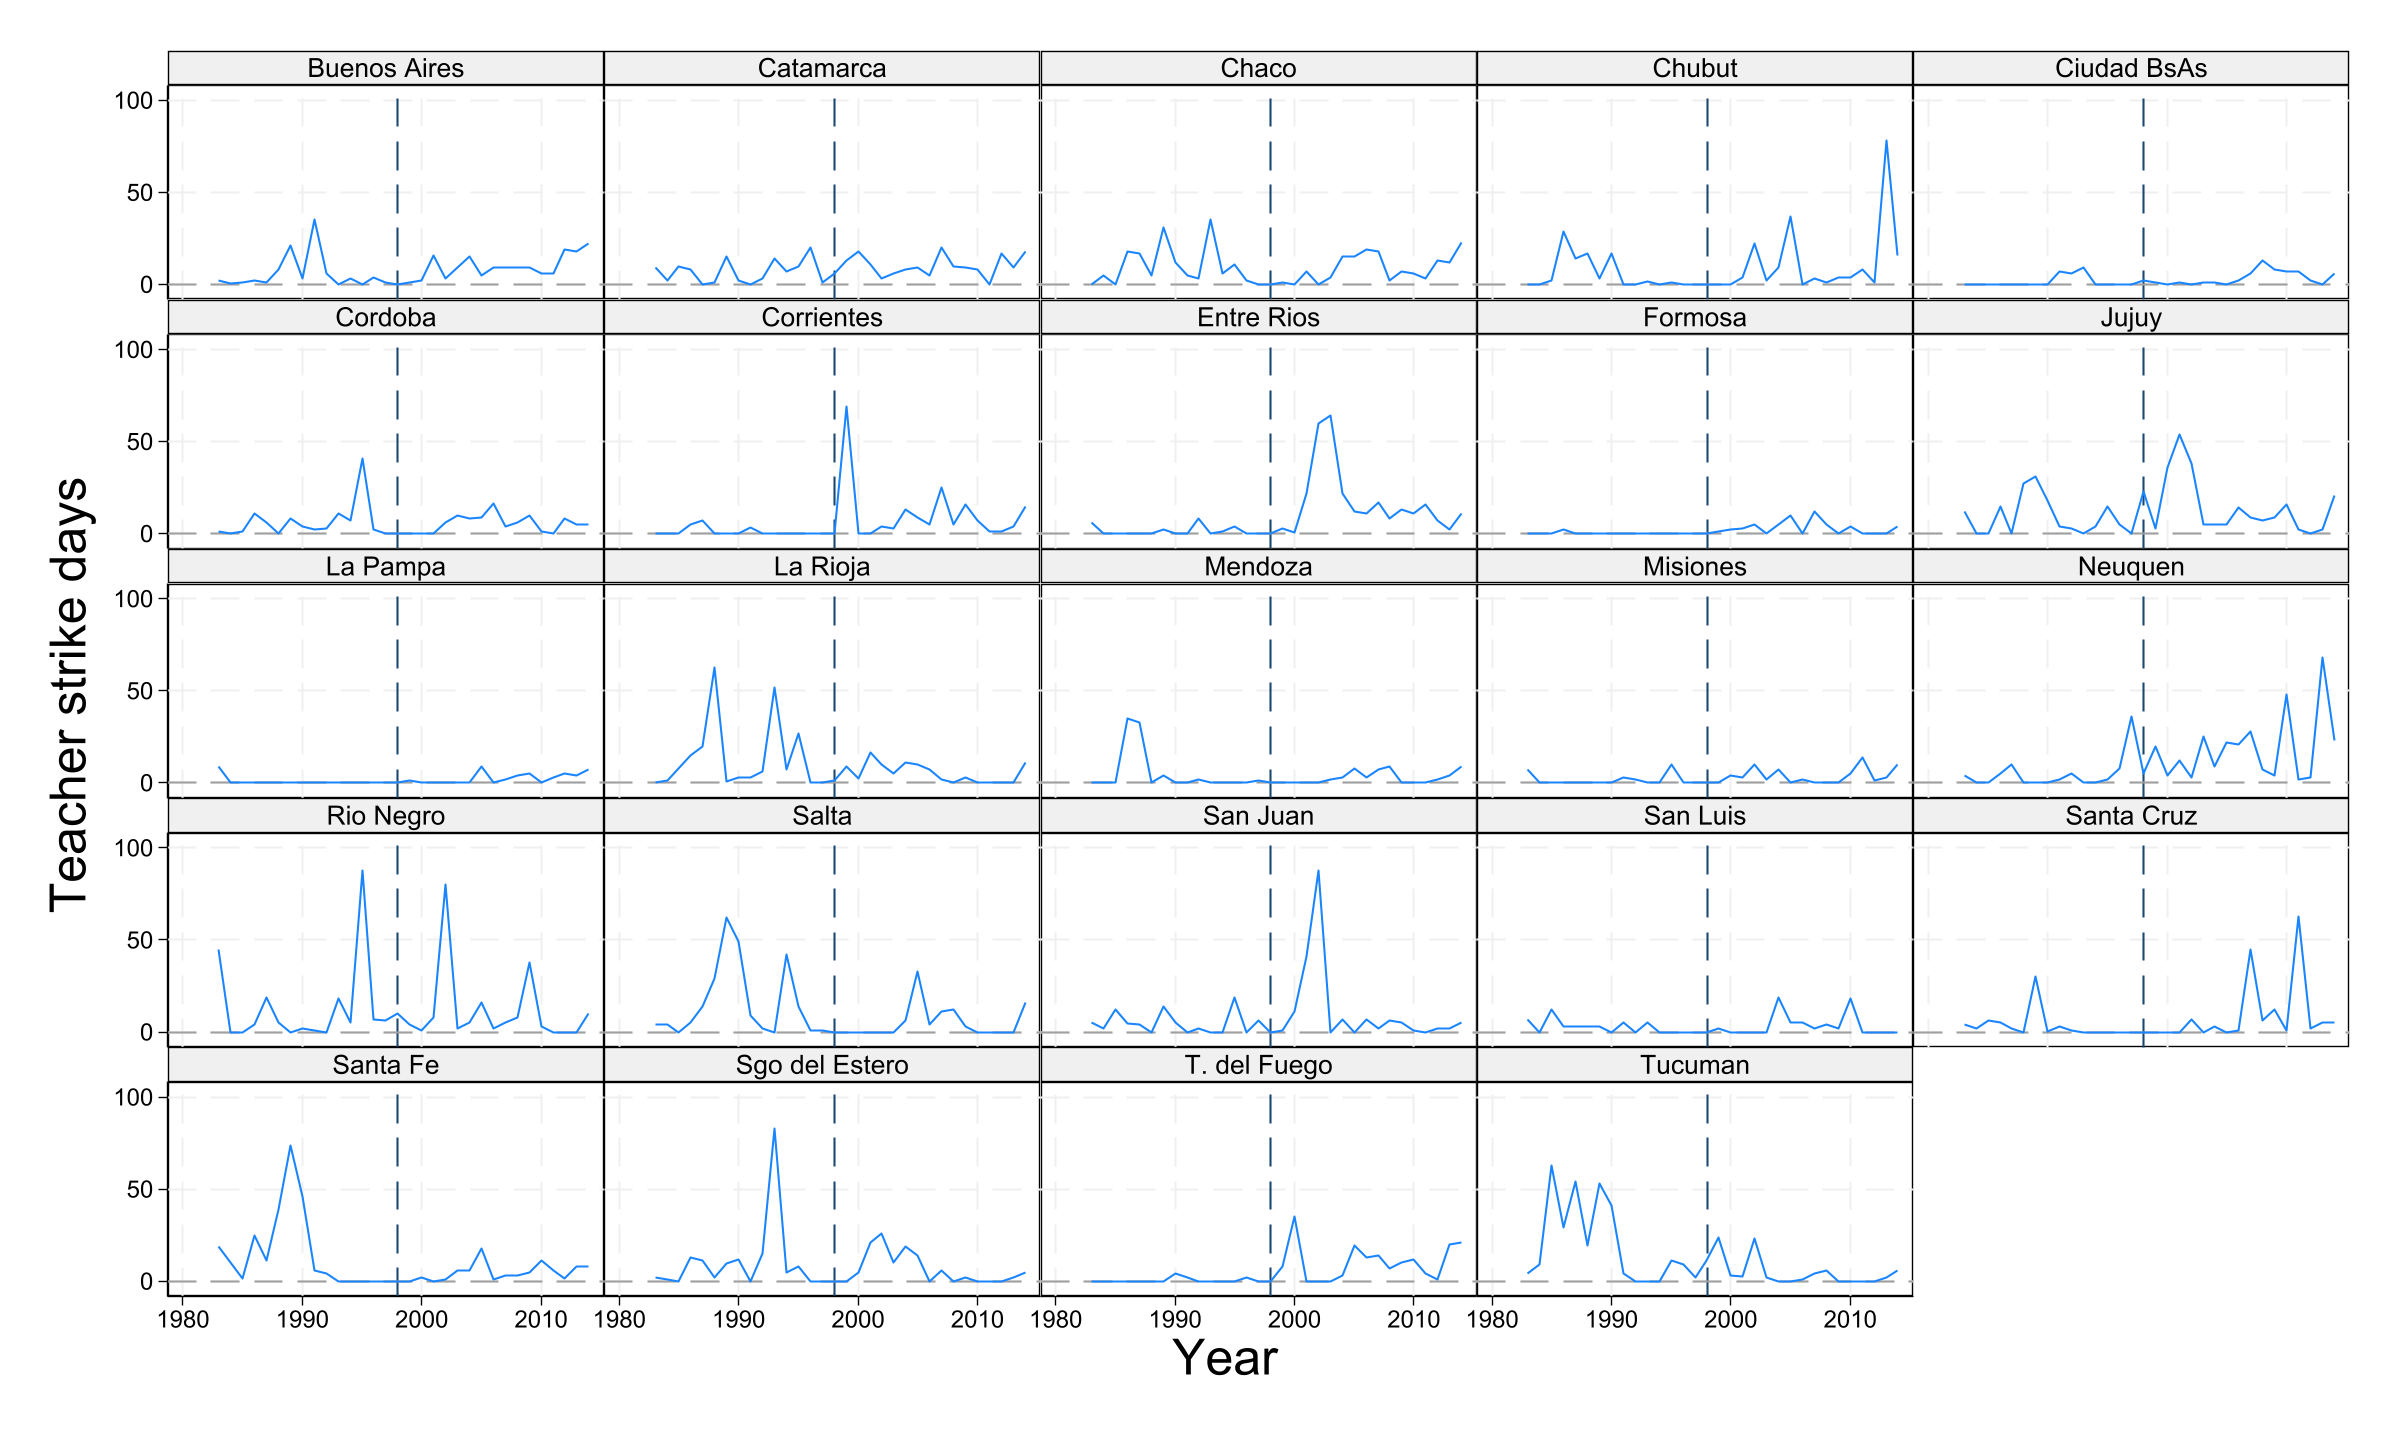
\includegraphics[width=0.95\textwidth]{../figures/Figure2A.png}\caption{Figure 2A}\end{figure}
\begin{figure}[!htbp]\centering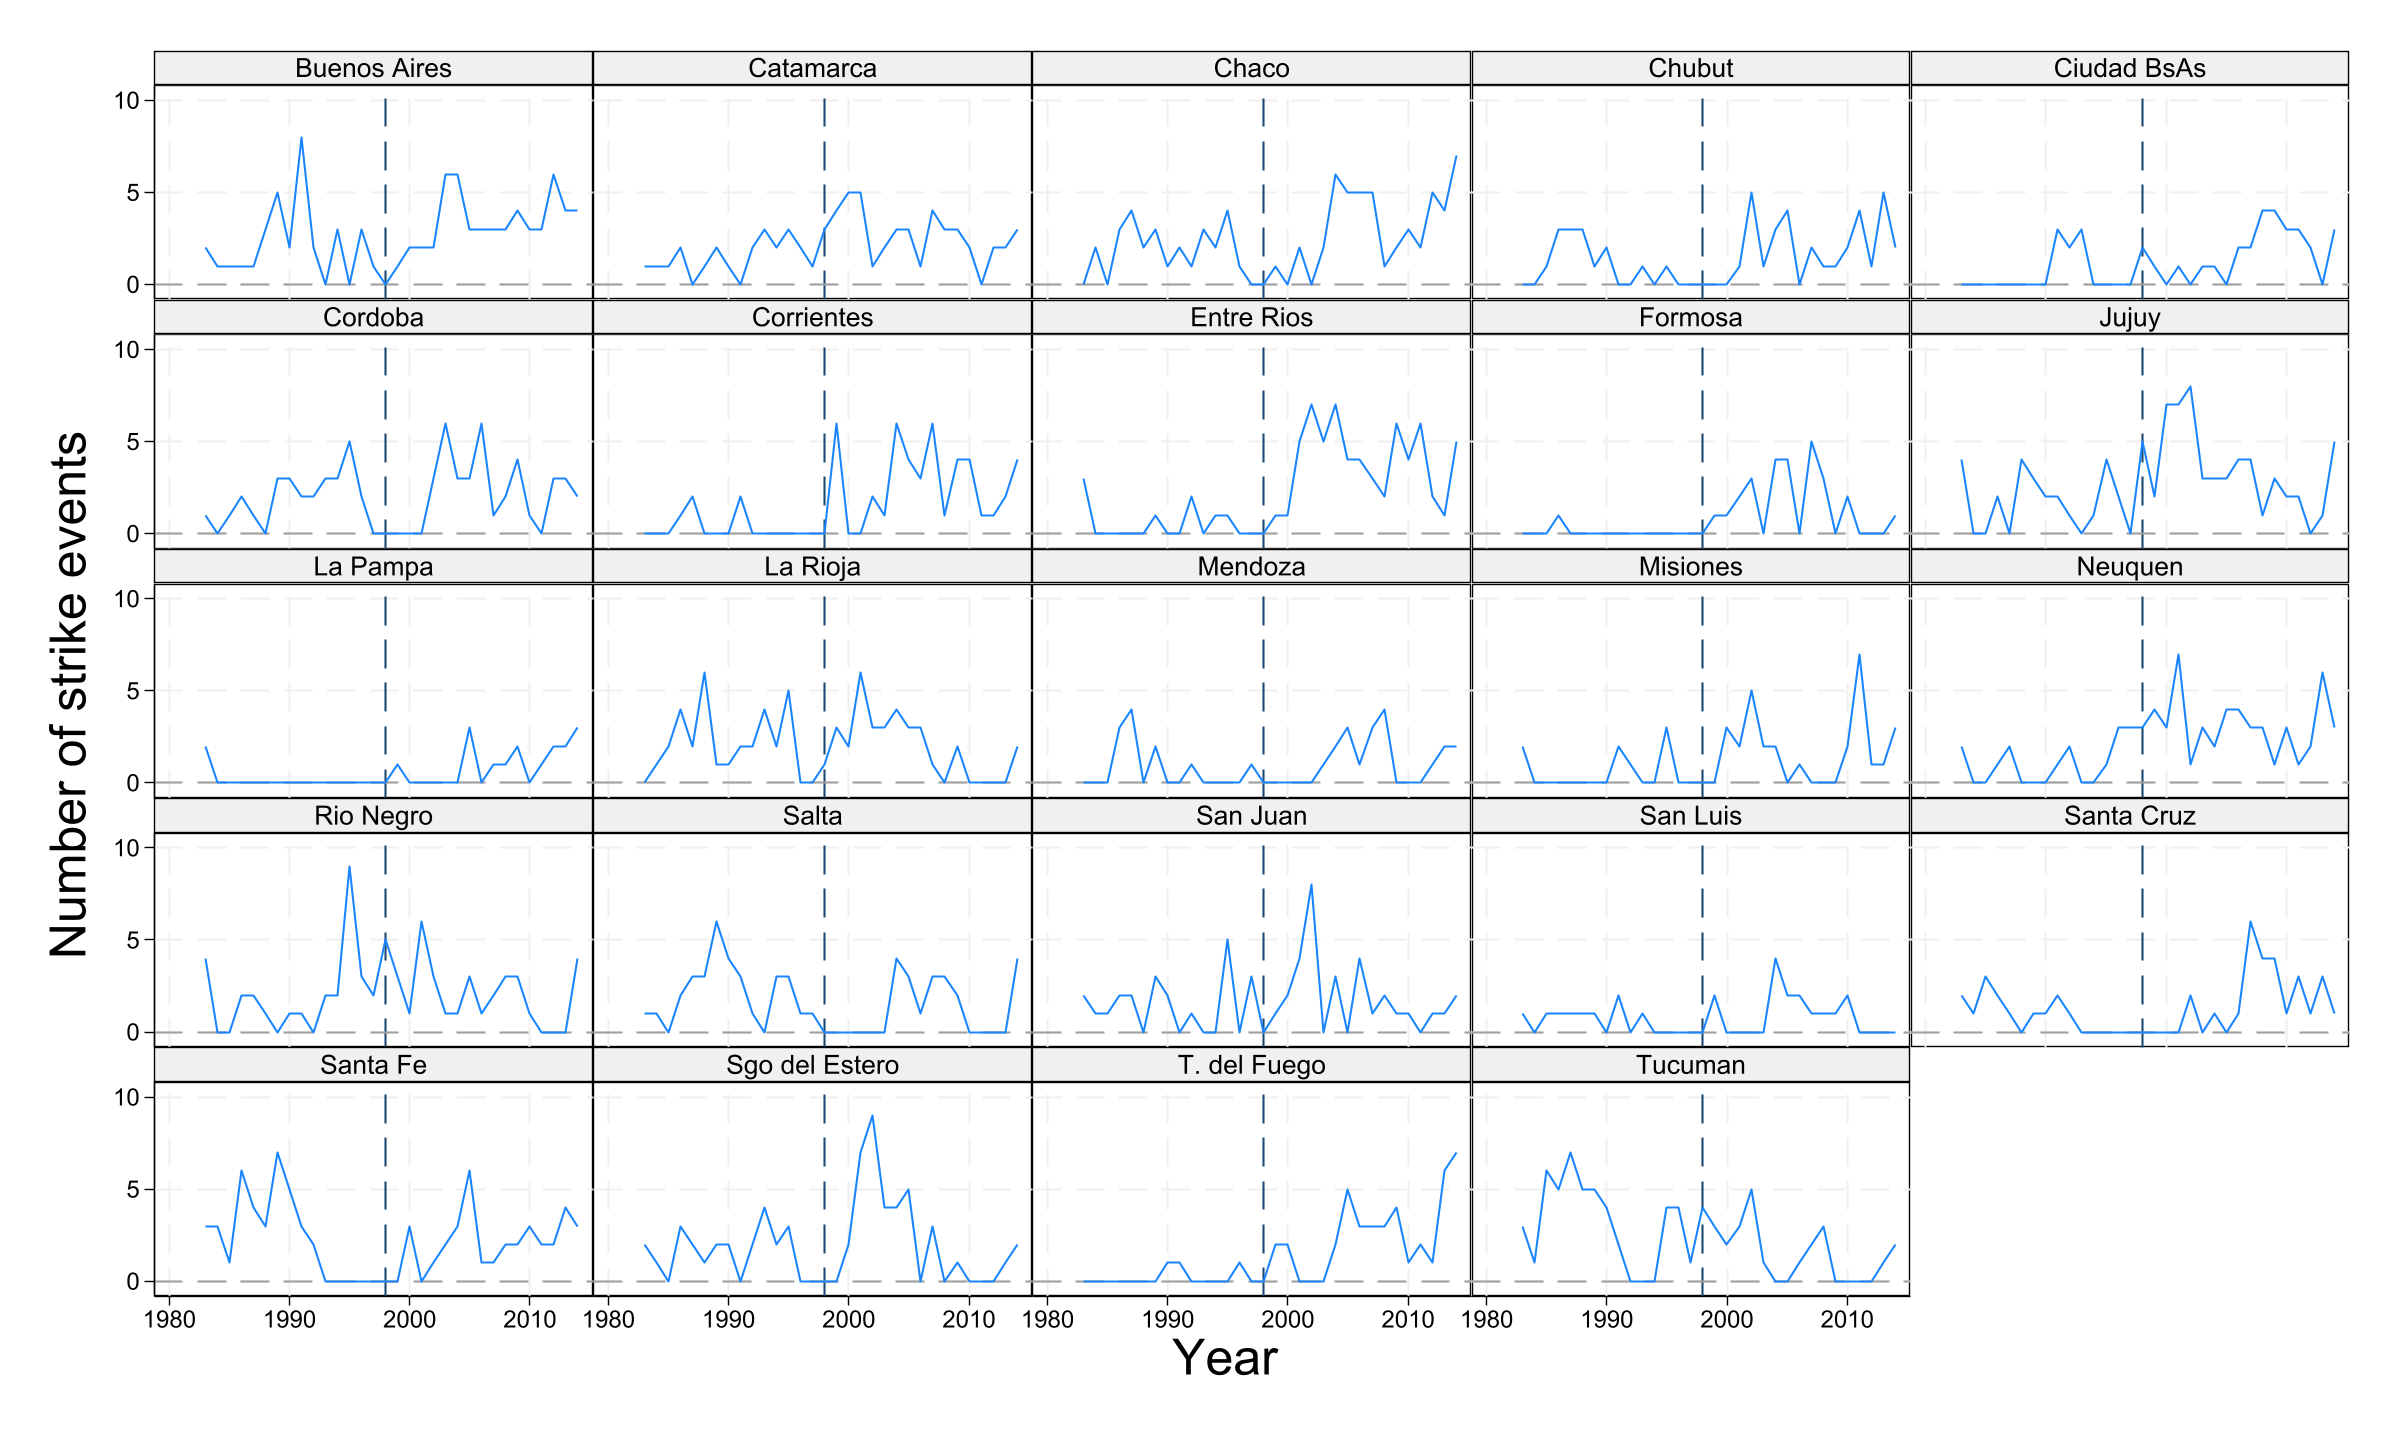
\includegraphics[width=0.95\textwidth]{../figures/Figure2B.png}\caption{Figure 2B}\end{figure}
\begin{figure}[!htbp]\centering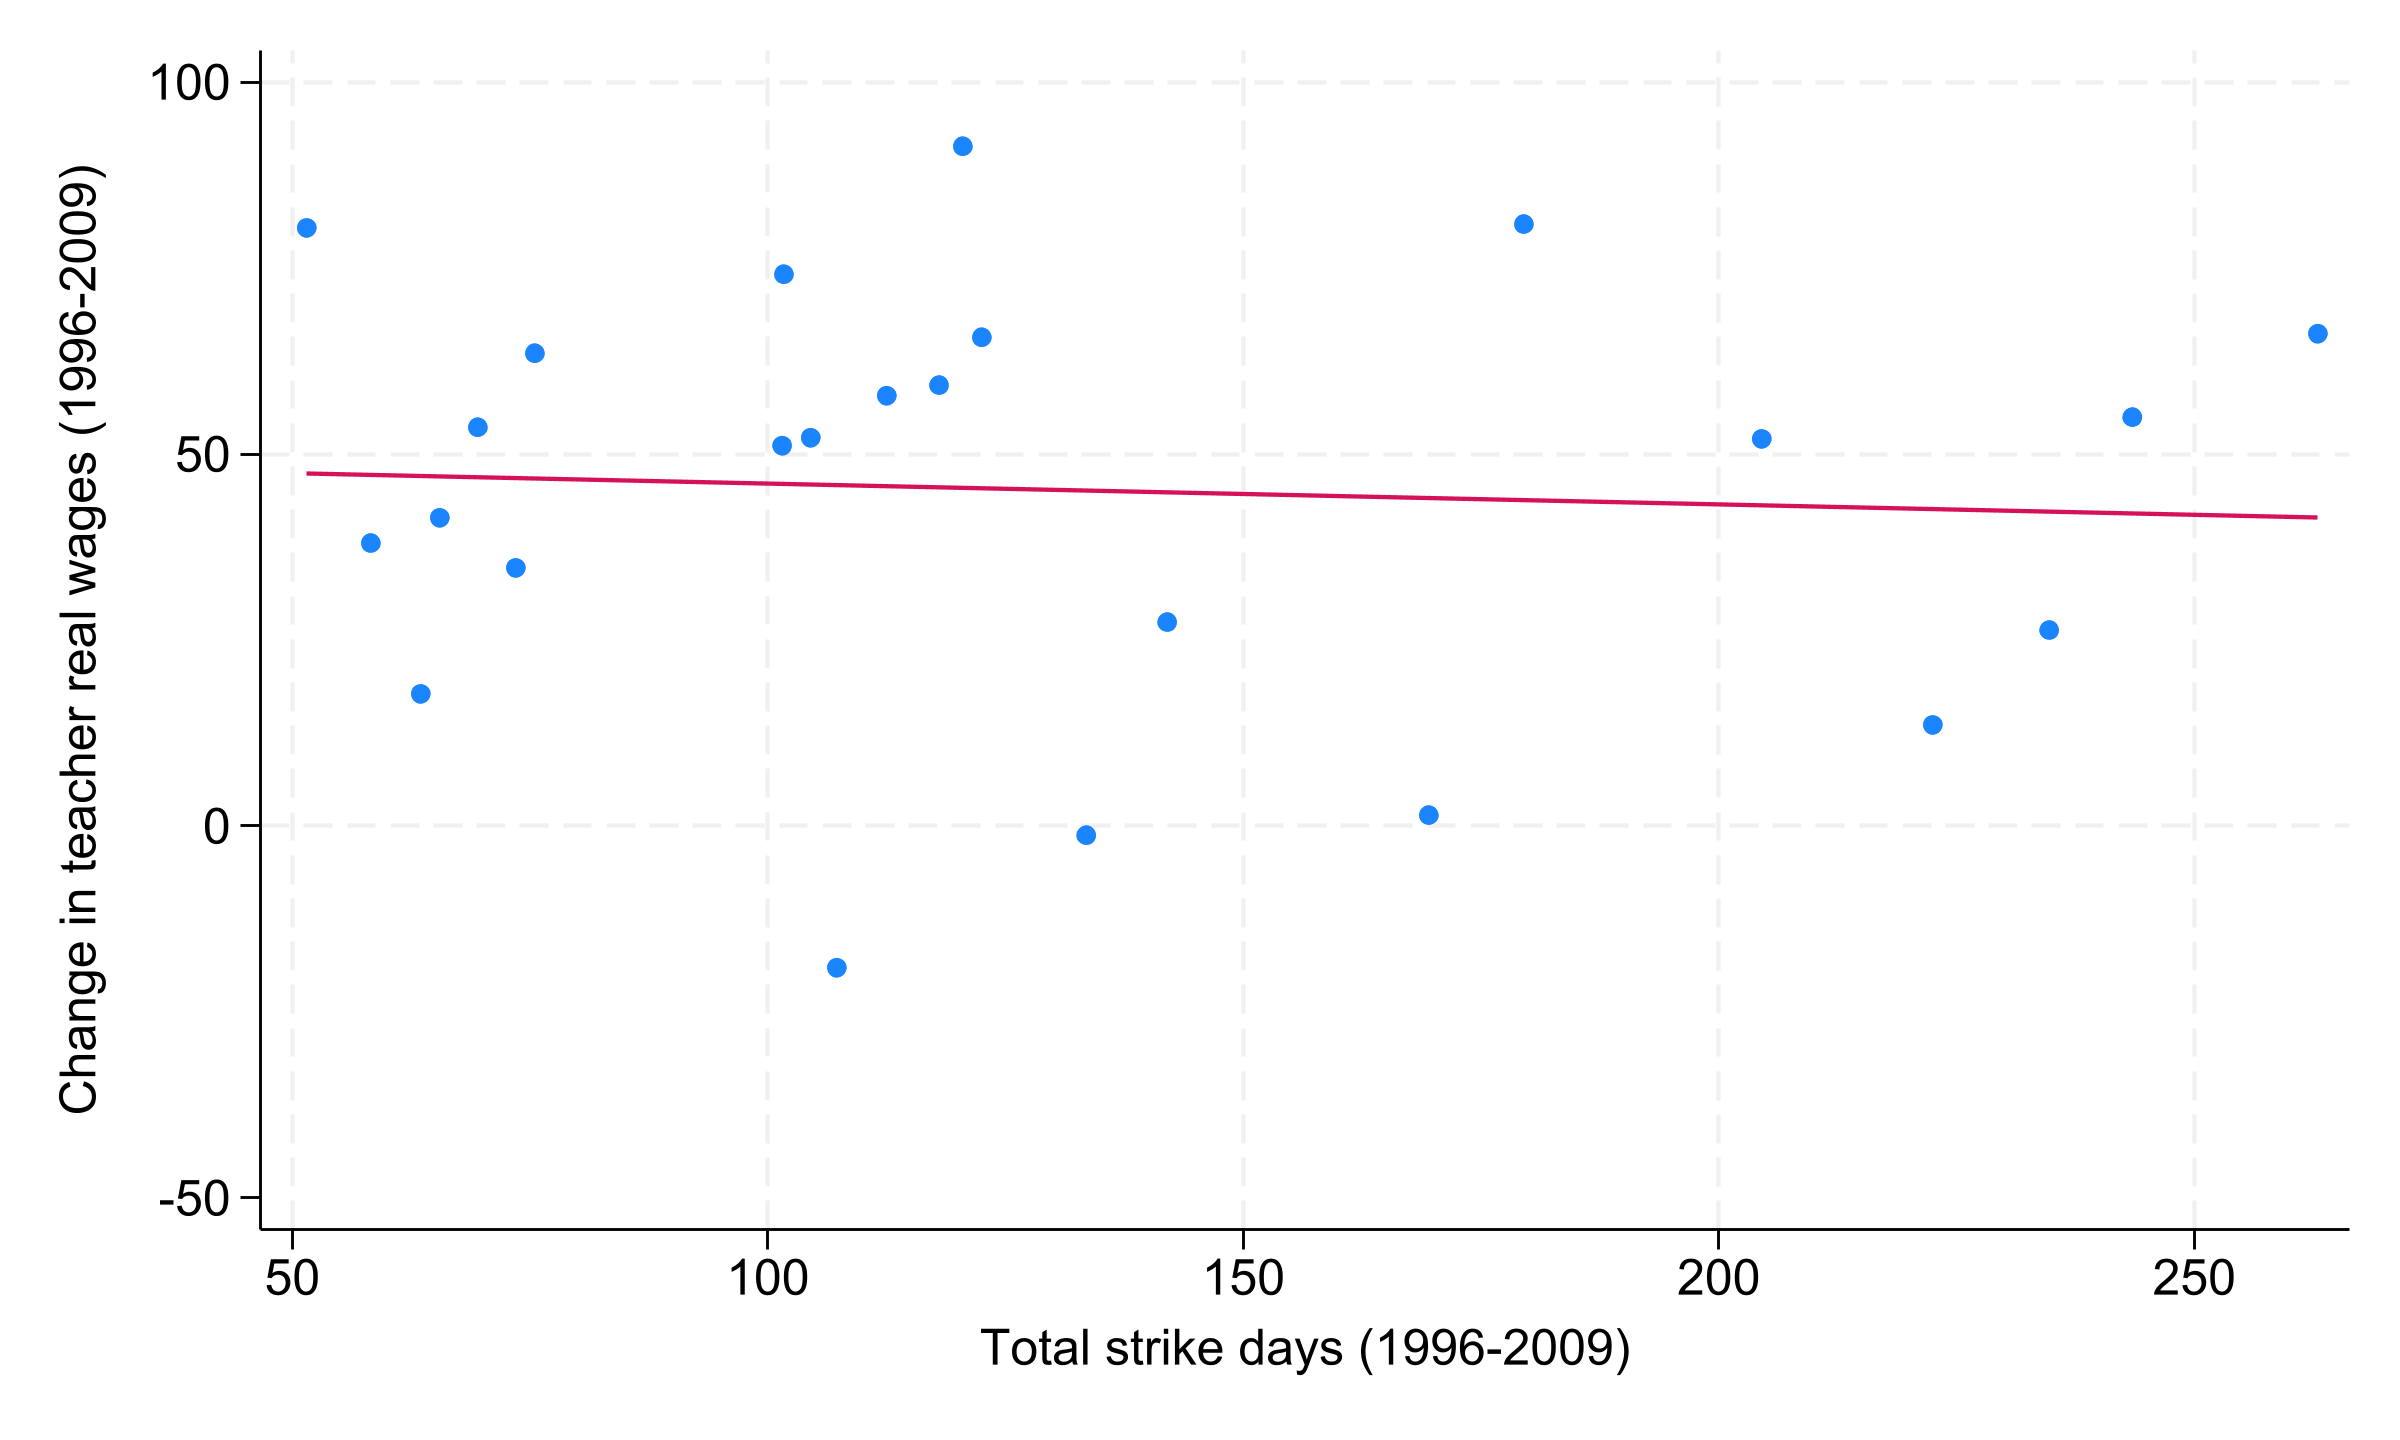
\includegraphics[width=0.95\textwidth]{../figures/FigureA1.png}\caption{Figure A1}\end{figure}
\clearpage
\section*{Presentation Figures}
\begin{figure}[!htbp]\centering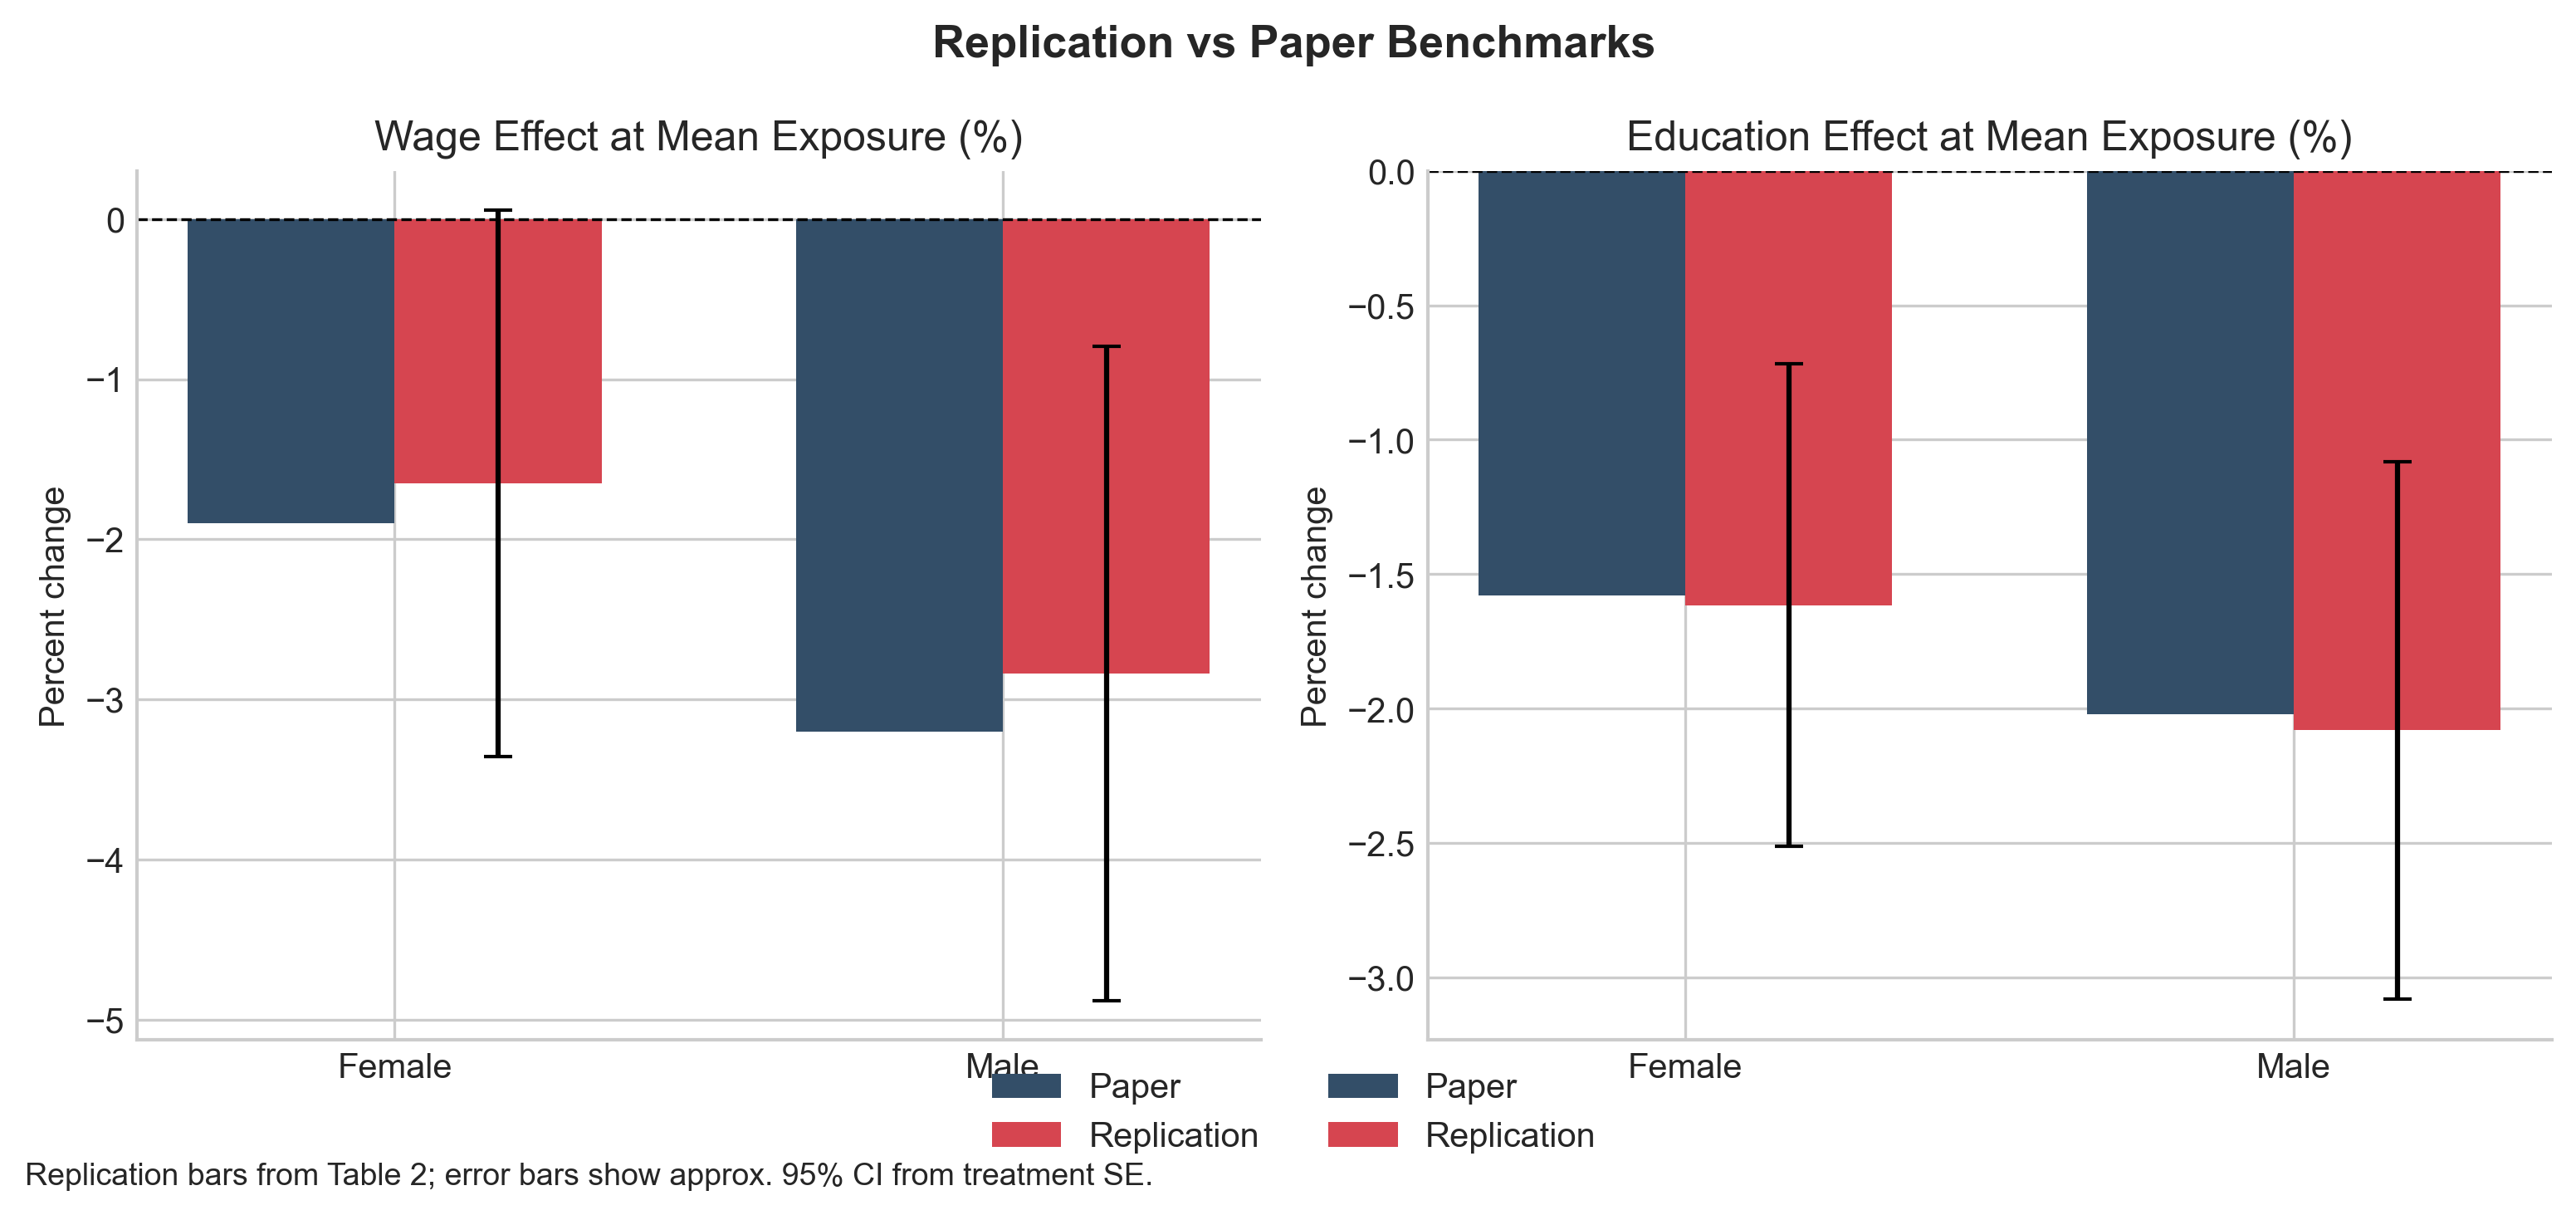
\includegraphics[width=0.9\textwidth]{../slides/fig_summary_effects.png}\caption{Summary effects}\end{figure}
\begin{figure}[!htbp]\centering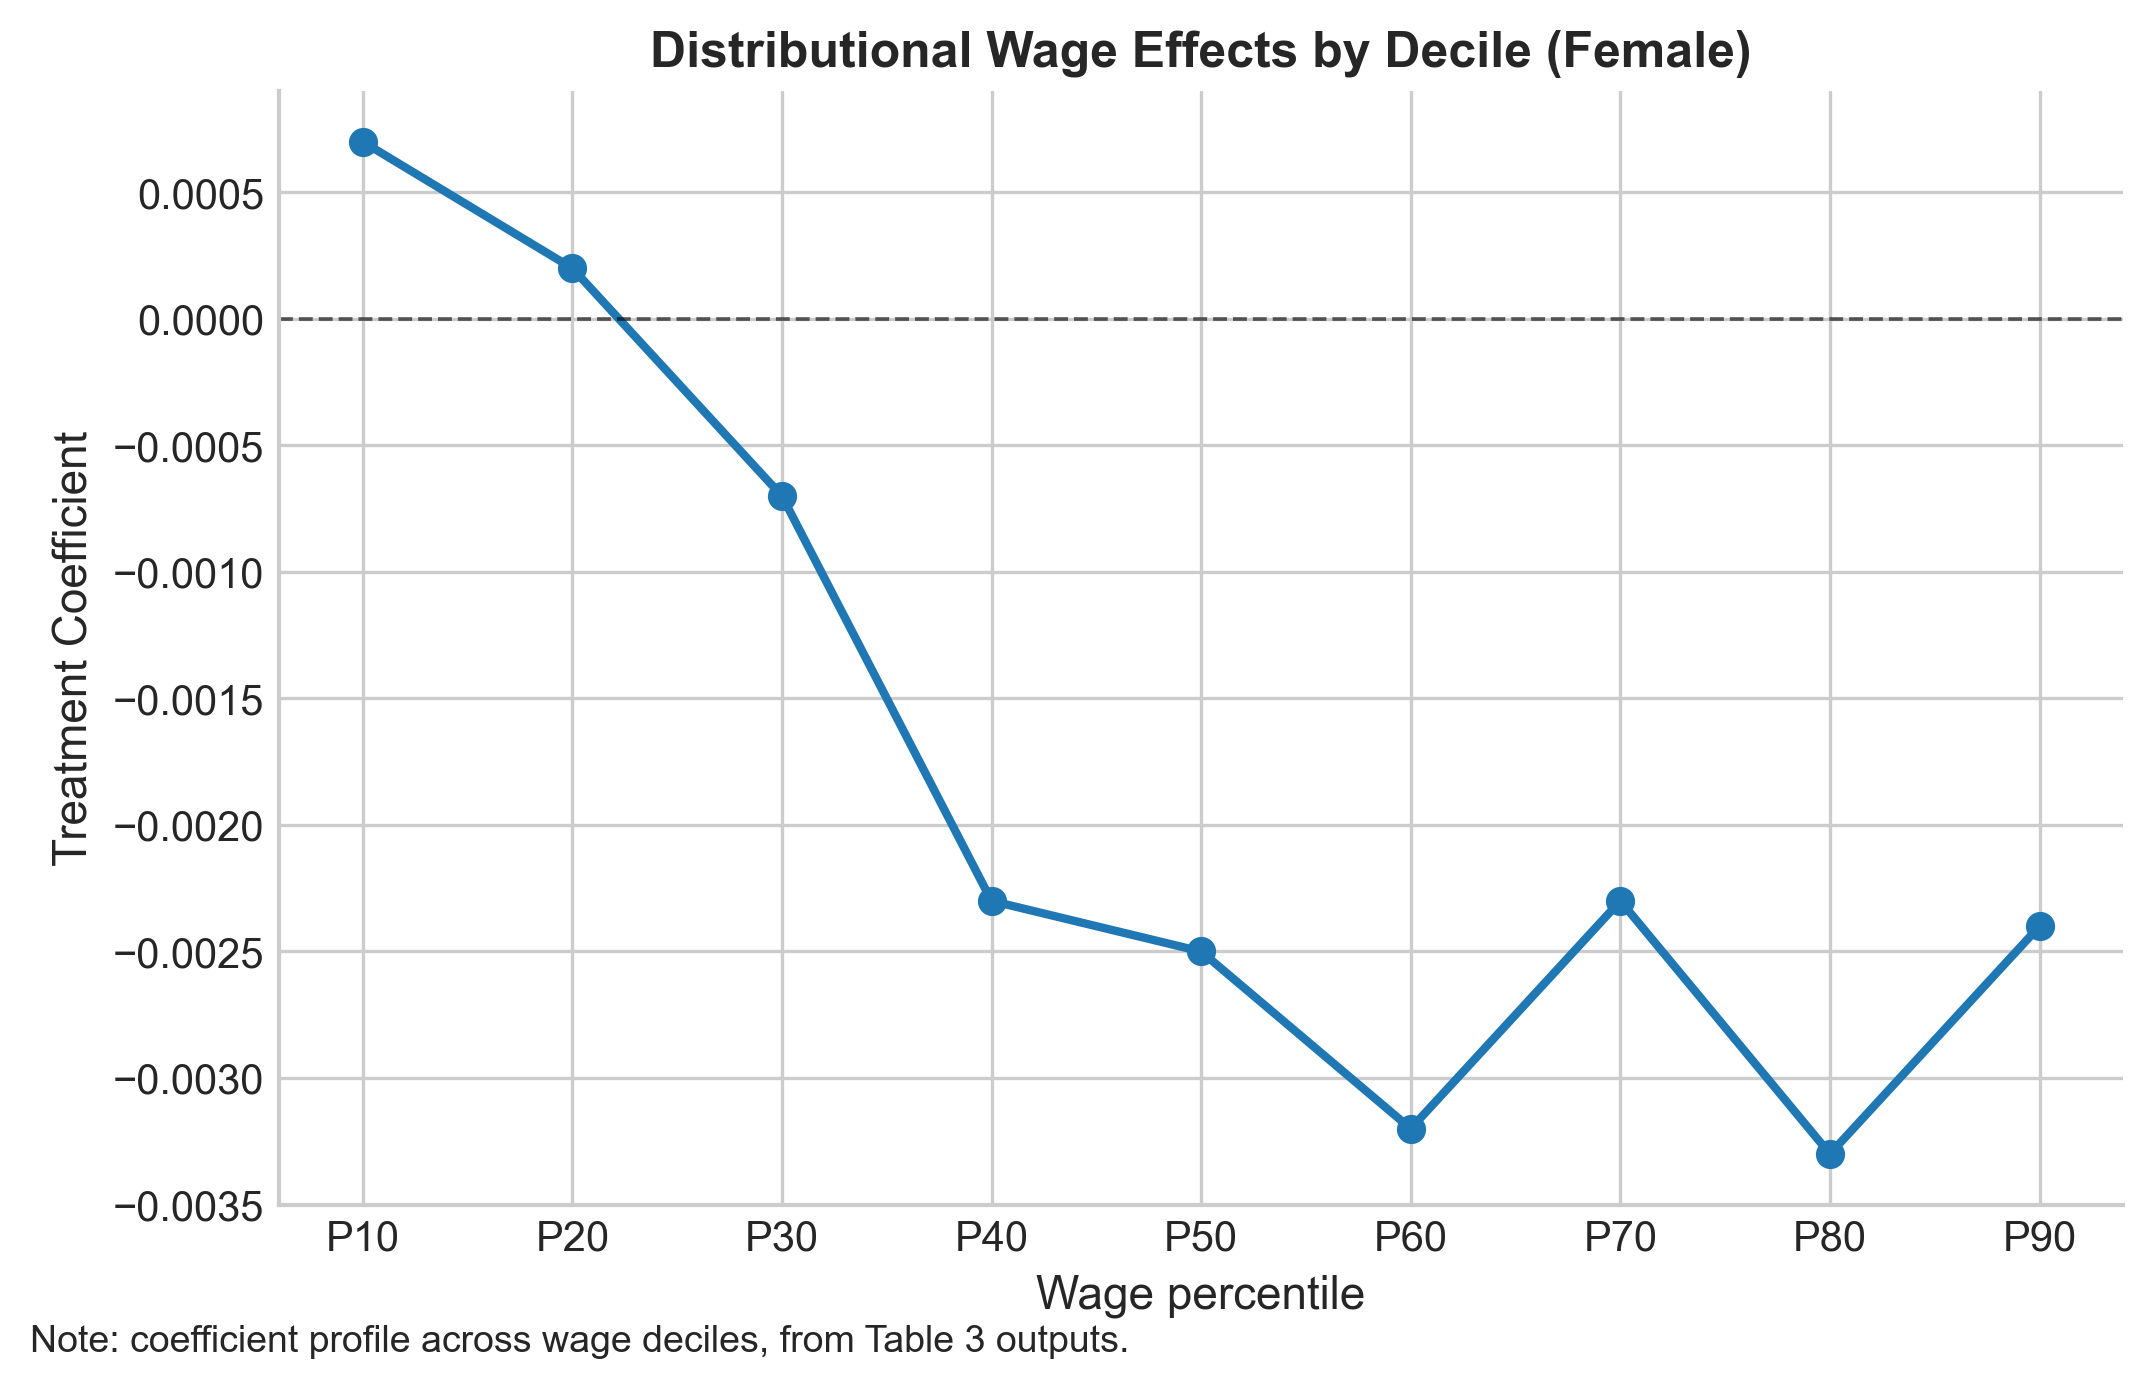
\includegraphics[width=0.9\textwidth]{../slides/fig_distributional_wage_female.png}\caption{Distributional wage effects (female)}\end{figure}
\begin{figure}[!htbp]\centering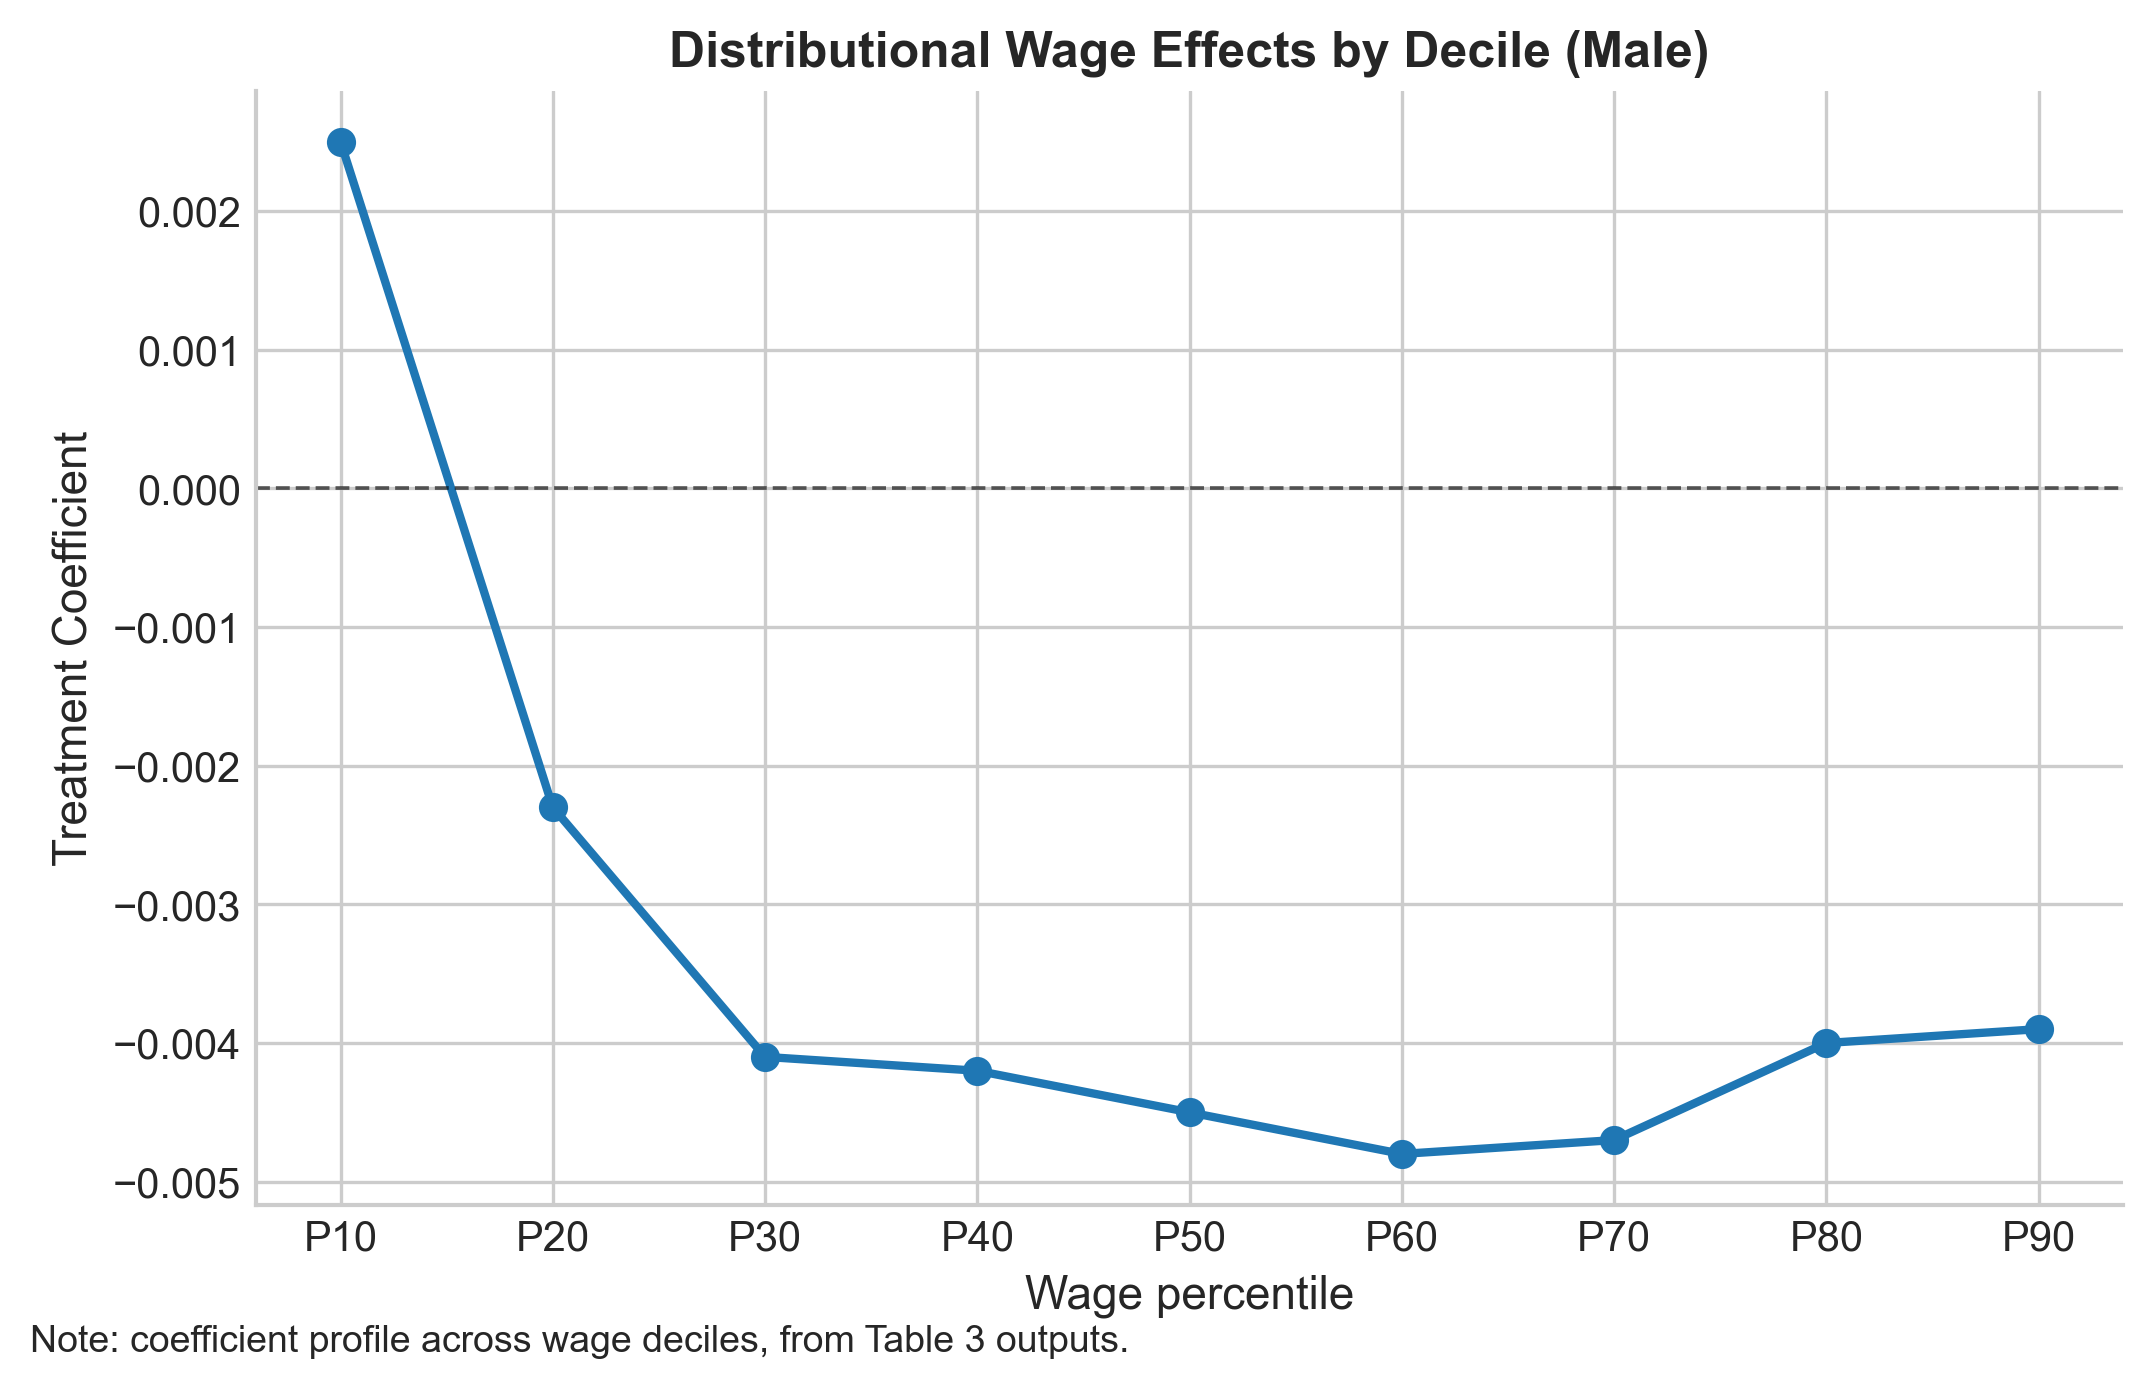
\includegraphics[width=0.9\textwidth]{../slides/fig_distributional_wage_male.png}\caption{Distributional wage effects (male)}\end{figure}
\end{document}
